\documentclass[11pt, a4paper]{report}

% Essential Packages
\usepackage[utf8]{inputenc}
\usepackage{geometry}
\geometry{
  a4paper,
  margin=2.54cm,
  headheight=14pt
}
\usepackage{graphicx}
\usepackage{float}
\usepackage{siunitx}
\usepackage{amsmath}
\usepackage{titlesec}
\usepackage{booktabs}
\usepackage{tabularx} 
\newcolumntype{L}{>{\raggedright\arraybackslash}X}
\newcolumntype{C}{>{\centering\arraybackslash}X}
\newcolumntype{R}{>{\raggedleft\arraybackslash}X}
\usepackage{makecell}
\usepackage{caption}
\usepackage{subcaption}
\usepackage{setspace}
\usepackage{fancyhdr}
\usepackage{parskip}
\setlength{\parindent}{0pt}
\setlength{\parskip}{6pt}
\usepackage{hyperref}
\usepackage{cite}
\usepackage{xcolor}
\usepackage{mdframed}
\usepackage{newtxtext,newtxmath} % Professional Times New Roman style
\usepackage{tocloft} % For TOC formatting
\usepackage{pgfgantt}
\usepackage{pdflscape}

% Adjust chapter title formatting to Arial equivalent (Helvetica)
% Using 'hang' to keep it on one line as per template requirements for Abstract/TOC
\titleformat{\chapter}[hang]
  {\fontfamily{phv}\fontsize{16}{18.4}\bfseries\selectfont}{\thechapter}{0.63cm}{}
\titleformat{name=\chapter,numberless}[hang]
  {\fontfamily{phv}\fontsize{16}{18.4}\bfseries\selectfont}{}{0pt}{}
\titlespacing*{\chapter}{0pt}{-20pt}{12pt}

% Adjust Section/Subsection according to guidelines
% Section: Arial Bold 16, 1.15 spacing, 12pt before/after, Indent 0 hanging 0.63cm
\titleformat{\section}[hang]
  {\fontfamily{phv}\fontsize{16}{18.4}\bfseries\selectfont}{\thesection}{0.63cm}{}
\titlespacing*{\section}{0pt}{12pt}{12pt}

% Subsection: Cambria Bold Italic 14, 1.5 spacing, 6pt before/after, Indent 0.63cm left hanging 0.76cm
% Using Times New Roman equivalent for Cambria to keep serif consistency in pdfLaTeX
\titleformat{\subsection}[hang]
  {\rmfamily\fontsize{14}{21}\bfseries\itshape\selectfont}{\thesubsection}{0.76cm}{}
\titlespacing*{\subsection}{0.63cm}{6pt}{6pt}

% TOC Formatting
\renewcommand{\cfttoctitlefont}{\fontfamily{phv}\fontsize{16}{18.4}\bfseries\selectfont}
\setlength{\cftbeforetoctitleskip}{12pt}
\setlength{\cftaftertoctitleskip}{0pt}
\setlength{\cftparskip}{10pt} % Paragraph spacing 10pt after for TOC entries
\renewcommand{\cftchapfont}{\rmfamily\fontsize{11}{13.2}\selectfont}
\renewcommand{\cftchappagefont}{\rmfamily\fontsize{11}{13.2}\selectfont}
\renewcommand{\cftsecfont}{\rmfamily\fontsize{11}{13.2}\selectfont}
\renewcommand{\cftsecpagefont}{\rmfamily\fontsize{11}{13.2}\selectfont}
\renewcommand{\cftsubsecfont}{\rmfamily\fontsize{11}{13.2}\selectfont}
\renewcommand{\cftsubsecpagefont}{\rmfamily\fontsize{11}{13.2}\selectfont}
\cftsetindents{chapter}{0cm}{1.5em}
\cftsetindents{section}{0cm}{2.3em}
\cftsetindents{subsection}{0.39cm}{3.2em}

\graphicspath{{figures/}}

% Academic Line Spacing (Text: 1.15)
\setstretch{1.15}

% Header and Footer setup
\pagestyle{fancy}
\fancyhf{}
\fancyhead[R]{\thepage}
\fancyhead[L]{ECM3175 Final Report}

\begin{document}

% Front Matter (Title Pages)
% ==========================================
% FRONT SHEET
% ==========================================
\begin{titlepage}
    \centering
    % Line 2: University of Exeter colour logo (3.81cm height, 9.26cm width)
    \vspace*{0.5cm} % Adjusting top to approximate Line 2
    
\includegraphics[width=9.26cm,height=3.81cm,keepaspectratio]{exeter_logo.png}\par
    
    % Line 6: Final Report
    \vspace{1.5cm}
    {\fontfamily{phv}\fontsize{24}{27.6}\bfseries\selectfont Final Report\par}
    
    % Line 10: project title
    \vspace{2cm}
    {\fontfamily{phv}\fontsize{15}{15}\bfseries\selectfont Finite Element Analysis of Sustainable Material Alternatives for Construction Helmet Shells under EN 397 Impact Conditions\par}
    
    % Line 11: student name
    \vspace{0.5cm}
    {\fontfamily{phv}\fontsize{15}{15}\bfseries\selectfont Mohammad Danish Basith Bin Haji Abu Bakar\par}
    
    % Line 15: 3rd Year Individual Project
    \vspace{2cm}
    {\fontfamily{phv}\fontsize{12}{13.8}\selectfont 3rd Year Individual Project\par}
    \vspace{10pt} % 10pt after
    
    \vfill
    
    % Lines 20 and 21: Declaration text
    \begin{flushleft}
    {\rmfamily\fontsize{11}{12.65}\selectfont I certify that all material in this thesis that is not my own work has been identified and that no material has been included for which a degree has previously been conferred on me.\par}
    \end{flushleft}
    
    % Line 27: Signed
    \vspace{2.5cm}
    \begin{flushleft}
    {\fontfamily{phv}\fontsize{12}{13.8}\bfseries\selectfont Signed..............................................................................................................\par}
    \end{flushleft}
    
    \vfill
    
    % Lines 33 and 34
    {\fontfamily{phv}\fontsize{11}{11}\selectfont College of Engineering, Mathematics, and Physical Sciences\par}
    \vspace{0.2cm}
    {\fontfamily{phv}\fontsize{11}{11}\selectfont University of Exeter\par}
\end{titlepage}

% ==========================================
% SECONDARY TITLE PAGE
% ==========================================
\begin{titlepage}
    \centering
    \vspace*{2cm} % Approx Line 4
    
    {\fontfamily{phv}\fontsize{30}{45}\selectfont Final Report\par}
    
    {\fontfamily{phv}\fontsize{20}{30}\selectfont ECM3175\par}
    
    \vspace{2.5cm} % Approx Line 10
    \begin{flushleft}
    {\fontfamily{phv}\fontsize{18}{20.7}\selectfont
    \textbf{Title:} Finite Element Analysis of Sustainable Material Alternatives for Construction Helmet Shells under EN 397 Impact Conditions\\
    \vspace{1cm} % Approx Line 13
    \textbf{Date of submission:} \today \\
    \vspace{1.5cm} % Approx Line 17
    \textbf{Student Name:} Mohammad Danish Basith Bin Haji Abu Bakar\\
    \textbf{Programme:} BEng Mechanical Engineering\\
    \textbf{Student number:} 720039833\\
    \textbf{Candidate number:} 306603\\
    \vspace{1.5cm} % Approx Line 24
    \textbf{Supervisor:} Dr. Khurram Wadee\par}
    \end{flushleft}
\end{titlepage}


% Abstract and Tables
\pagenumbering{roman}
\chapter*{Abstract}
\addcontentsline{toc}{chapter}{Abstract}

\begingroup
\setstretch{1.0}
\rmfamily\fontsize{11}{11}\itshape\selectfont
\setlength{\parskip}{6pt}

This investigation evaluates the structural performance of sustainable polymer 
al\-tern\-at\-ives, specifically Recycled Poly\-car\-bon\-ate (rPC) and a 
Bamboo-HDPE 30\% wt composite, against standard Virgin High-Density 
Polyethylene (HDPE) and ABS safety helmets. Designed to meet the EN 397 industrial 
safety standard, construction helmets must restrict the transmitted force 
to a 5.0 kg headform to a maximum of 5.0 kN under a 49 Joules impact. 
Applying LS-DYNA explicit finite element analysis (FEA), the simulations 
modeled an upward relative impact velocity of 4.43 m/s based on the 
principle of Galilean Invariance.

A five-phase analytical methodology concluded with an advanced 30$^\circ$ 
oblique impact simulation to quantify rotational kinematics. 
Thermodynamic validation confirmed computational stability with 
exactly 0\% hourglass energy across all material models. Comparison of 
raw nodal acceleration data to filtered SAE J211 CFC 60 signals isolated the 
true macroscopic structural deceleration from numerical contact noise.

Results identified two primary energy-absorption mechanisms: highly ductile 
polymers (HDPE) absorbed impact energy through internal strain yielding, 
while high-modulus materials (ABS, rPC) used load distribution due to 
increased flexural stiffness to distribute impact forces across a wider surface area of the 
EPS liner. The Recycled PC shell demonstrated superior 
performance in oblique loading, achieving a 74\% reduction in peak 
rotational acceleration compared to Virgin HDPE. This is attributed to 
reduced tangential frictional interaction, where the higher flexural modulus 
limits localized surface deformation and reduces tangential torque compared 
to the plastic deformation observed in HDPE.

The findings confirm that sustainable material alternatives provide 
sufficient structural protection and meet safety-critical regulatory requirements while 
significantly reducing the environmental footprint of PPE production.\par
\endgroup

\vspace{12pt}
\noindent{\rmfamily\fontsize{12}{13.8}\itshape\selectfont \textbf{Keywords:} Explicit Dynamics, EN 397, FEA, Sustainable Polymers, Impact Analysis, SAE J211, Oblique Impact, Rotational Kinematics\par}


\newpage
\tableofcontents
\newpage
\listoffigures
\newpage
\pagenumbering{arabic}

% Main Chapters
\chapter{Introduction and Background}

\section{Background and Motivation}
Industrial safety helmets are critical personal protective equipment (PPE) 
designed to shield workers from traumatic brain injury caused by falling 
objects \cite{long2015, mishra2021}. Their protective function relies heavily on shell deformation, liner 
compression, and energy distribution during an impact event. Traditionally, 
these shells are injection-moulded from petroleum-derived engineering 
thermoplastics such as Virgin High-Density Polyethylene (HDPE), Acrylonitrile 
Butadiene Styrene (ABS), and Polycarbonate. These materials offer reliable 
performance, high impact resistance, and cost-effectiveness. However, stricter 
environmental regulations and the shift towards a circular economy now 
necessitate sustainable material alternatives that remain compliant with strict 
safety standards \cite{yadav2024}.

\section{The EN 397 Standard}
The European Standard EN 397 (DIN EN 397) represents the standardized safety 
specification for industrial safety helmets \cite{en397}. This standard mandates specific 
design requirements, performance specifications, and testing methodologies. 
The primary shock absorption test requires a helmet to be mounted on a 
standardized aluminium headform (per EN 960 specifications \cite{en960}). A hemispherical 
striking mass of 5.0 kg is dropped from a 1-metre height onto the helmet 
crown, imparting approximately 49 Joules of kinetic energy. To achieve 
certification, the maximum transmitted force recorded at the neck of the 
headform must not exceed 5.0 kN.

\section{Project Aims and Objectives}
The primary objective of this project is to evaluate the performance of 
construction helmet shells under EN 397 impact conditions and establish 
criteria that support the adoption of sustainable materials. The specific 
objectives are:
\begin{itemize}
    \item To establish baseline impact performance metrics for conventional 
    HDPE and ABS polymers using ANSYS LS-DYNA explicit finite element 
    simulation \cite{lsdyna2021}.
    \item To simulate and evaluate sustainable alternatives: a Bamboo-HDPE 
    30\% wt composite and Recycled Polycarbonate (rPC).
    \item To quantify macroscopic force transmission, energy absorption 
    kinematics, and microscopic stress distribution across the different 
    material properties.
    \item To validate the explicit dynamics simulation thermodynamically and 
    apply appropriate signal processing (SAE J211 \cite{sae1995}) to extract physical data.
\end{itemize}

The selected objectives establish a systematic performance evaluation of sustainable alternatives. Baseline HDPE and ABS models provide the validated reference against EN 397 experimental data required before introducing the previously unquantified response of Bamboo-HDPE and recycled Polycarbonate. Thermodynamic validation and SAE J211 signal processing address the numerical instability common in explicit FEA, ensuring that the final comparative metrics isolate structural behavior from computational noise.


\section{Scope and Assumptions}

This study is concerned with the macroscopic structural deceleration and 
force transmission of construction helmet shells under normal crown 
impact (4.43~m/s) and advanced 30$^\circ$ oblique impact conditions. To 
maintain computational focus on shell material performance, several 
simplifying assumptions were implemented:
\begin{itemize}
    \item \textbf{Geometry and Loading:} Impact includes a primary perpendicular (\texorpdfstring{0$^\circ$}{0 degrees}) drop onto the crown apex and a secondary \texorpdfstring{30$^\circ$}{30 degrees} oblique impact to assess rotational kinematics. To optimize the computational domain, these were modeled using a kinematic shift based on Galilean Invariance, where the helmet/headform assembly was assigned an initial upward velocity of 4.43 m/s against a stationary rigid ceiling. This approach isolates the impact event from unnecessary free-flight processing while maintaining standard mass parity.
    \item \textbf{Material Modelling:} The polymer shells are treated as bilinear isotropic materials. The energy-absorbing liner is modelled as linear-elastic Expanded Polystyrene (EPS). The headform is modelled as a perfectly rigid 5.0 kg sphere to simplify contact definitions and ensure computational efficiency while maintaining standard mass parity.
    \item \textbf{Environmental Factors:} All simulations are conducted at room temperature (\texorpdfstring{23~$^\circ$C}{23 degrees C}); temperature-dependent ductility and material aging are not considered.
\end{itemize}
The Bamboo-HDPE composite is approximated as an isotropic material, a simplification that is later addressed in the discussion of simulation limitations (see Section~\ref{sec:limitations}).

\chapter{Literature Review}

\section{Impact Stress Distribution and Mechanics}
Impact stress analysis on construction helmet shells is a critical engineering 
domain. Under EN 397 conditions, shells experience peak stresses concentrated 
at the dome apex. According to Long et al. \cite{long2015}, finite element 
models applying explicit solvers are effective at mapping these transient 
loads. However, a primary limitation in such models is the frequent 
adoption of simplified linear elastic material assumptions for the underlying 
foam liners, which may fail to capture the energy dissipation associated with 
non-linear cell crushing. Research indicates that standard HDPE shells 
experience peak stresses of 2.55--3.57 kg/mm$^2$ with moderate deformation, while ABS 
shells undergo peak stresses of 3.06--4.59 kg/mm$^2$ due to their higher stiffness.

While Wu et al. \cite{wu2022} report that helmet shells remain primarily 
within elastic deformation limits (strains of 4\%--6.3\%), there is 
substantial uncertainty regarding material response under high-strain-rate 
impact loading. Specifically, the energy absorption capacity is fundamentally 
dictated by the material's elastic modulus; however, the transition from 
structural yielding in ductile materials to load distribution in stiff 
materials is often treated as a binary mechanism. This study identifies a 
critical gap in understanding how this transition influences transmitted 
impulse when sustainable, non-conventional polymers are introduced.

\section{Conventional Material Properties}
Conventional materials have dictated helmet design for decades, yet their 
comparative performance under varying impact velocities remains under-scrutinised.
\begin{itemize}
    \item \textbf{HDPE:} Widely used due to its semi-rigid nature and high 
    ductility. While industrial data suggests a yield strength of 
    approx.\ 2.55 kg/mm$^2$ \cite{cruz2023}, academic studies often 
    report conflicting results depending on the molecular weight and 
    processing conditions, indicating that standard HDPE performance may 
    vary measurably in field applications.
    \item \textbf{ABS:} Known for exceptional rigidity and tensile strength 
    (4.08--5.10 kg/mm$^2$). While Author A reports high energy absorption 
    in HDPE, Author B suggests reduced performance under transient loading, 
    indicating uncertainty in how flexural modulus (approx. 214.14 kg/mm$^2$) 
    interacts with the localized buckling resistance required for 
    EN 397 compliance.
\end{itemize}

\section{Sustainable and Environmentally Friendly Materials}
Environmental sustainability considerations are driving helmet material 
innovation, but existing research is primarily restricted to 
quasi-static contexts, which fail to represent the high-strain-rate 
environment of an industrial impact.
\begin{itemize}
    \item \textbf{Bio-Based Polymers:} Materials such as Bio-PE offer 
    potential impact resistance equivalent to fossil-derived PE \cite{alvarez2022}. 
    However, the lack of documented high-velocity impact data for these 
    renewable biomass feedstocks represents a major hurdle for regulatory 
    acceptance in safety-critical PPE.
    \item \textbf{Natural Fibre Composites:} Integrating bamboo or coir 
    fibres into thermoplastic matrices increases tensile strength 
    \cite{obele2015, chandramohan2015}. Research by Chen et al. \cite{chen2020} 
    suggests 10\% fibre loading is optimal; however, their study 
    focuses on tensile rather than impact dynamics. The structural 
    viability of higher loadings (up to 30\%) remains contested, 
    particularly regarding the interfacial bonding required to maintain 
    integrity under transient EN 397 loads.
    \item \textbf{Recycled Polycarbonate (rPC):} Studies indicate that rPC 
    can maintain performance parity with virgin filaments \cite{baechler2013}. 
    However, these studies often overlook the effects of polymer 
    degradation during multiple recycling cycles, which can induce 
    brittleness. While its extreme rigidity promotes reduced tangential 
    frictional interaction \cite{mills2011}, the potential for catastrophic 
    brittle fracture under peak EN 397 loads remains an unaddressed risk 
    in current literature.
\end{itemize}

While explicit FEA has benchmarked conventional safety helmets \cite{long2015, wu2022}, 
sustainable alternatives lack a validated high-velocity performance baseline. 
This investigation addresses this critical deficiency by establishing a 
comparative framework to quantify their kinetics and regulatory compliance 
under EN 397 transient loading, explicitly accounting for the uncertainties 
identified in existing literature.

\chapter{Methodology and Theory}

This chapter outlines the theoretical foundations of explicit dynamics and the specific mechanical principles governing the EN 397 drop test simulation.

\section{Explicit Dynamics Theory}
Explicit dynamics apply the central difference method to solve kinematic equations of motion directly without global stiffness matrix inversions. This is highly efficient for high-nonlinearity, millisecond-duration impact events.

\subsection{Central Difference Integration}
The semi-discrete equations of motion at time $t_n$ are expressed as:
\begin{equation}
    M \ddot{u}_n = F^{ext}_n - F^{int}_n
\end{equation}
where $M$ is the diagonal (lumped) mass matrix, $\ddot{u}_n$ is the nodal acceleration vector, $F^{ext}_n$ represents external applied loads (including contact forces), and $F^{int}_n$ represents internal nodal forces.

LS-DYNA employs a modified central difference time integration scheme (Leapfrog method) to advance the solution~\cite{lsdyna2021}. The nodal velocities and displacements are updated according to:
\begin{equation}
    \dot{u}_{n+1/2} = \dot{u}_{n-1/2} + \ddot{u}_n \Delta t_n
\end{equation}
\begin{equation}
    u_{n+1} = u_n + \dot{u}_{n+1/2} \Delta t_{n+1/2}
\end{equation}
where $\Delta t_{n+1/2} = \frac{1}{2}(\Delta t_n + \Delta t_{n+1})$. This explicit approach allows for efficient processing of complex contact interactions between the rigid headform, the EPS liner, the polymer shell, and the rigid ceiling.

\subsection{Stability and Time Step Control}
The central difference method is conditionally stable. The time step $\Delta t$ is strictly limited by the Courant-Friedrichs-Lewy (CFL) condition~\cite{belytschko2013}:
\begin{equation}
    \Delta t \leq \Delta t_{crit} = \frac{L_{min}}{c}
\end{equation}
where $L_{min}$ is the characteristic length of the smallest element in the mesh and $c$ is the local speed of sound in the material ($c = \sqrt{E/\rho}$). For this study, the 2 mm mesh resolution at the crown impact zone dictates the global time step, ensuring that the stress wave propagation is accurately captured during the 49 J impact.

\section{Unit System and Numerical Consistency}
A consistent [kg, mm, s] unit set was adopted for LS-DYNA stability. Strength and contact pressure are reported in kg/mm$^2$ ($1 \text{ kg/mm}^2 \approx 9.81 \text{ MPa}$), while Young’s ($E$) and Tangent ($E_{tan}$) Moduli are in GPa. Transmitted forces and impact energy use kN and J, respectively.
To optimise the computational domain and stabilise the explicit penalty contact 
algorithms, a kinematic shift was implemented based on the principle of 
Galilean Invariance. Rather than a transient drop of a 5.0 kg mass onto a 
stationary helmet, the rigid ``floor'' was modelled as a stationary ceiling. 
The helmet and the 5.0 kg spherical headform assembly were grouped and 
assigned a uniform upward initial velocity of 4.43 m/s. Figure~\ref{fig:assembly_setup} 
illustrates the numerical assembly and the kinematic boundary conditions.

\begin{figure}[H]
    \centering
    \begin{subfigure}[b]{0.45\textwidth}
        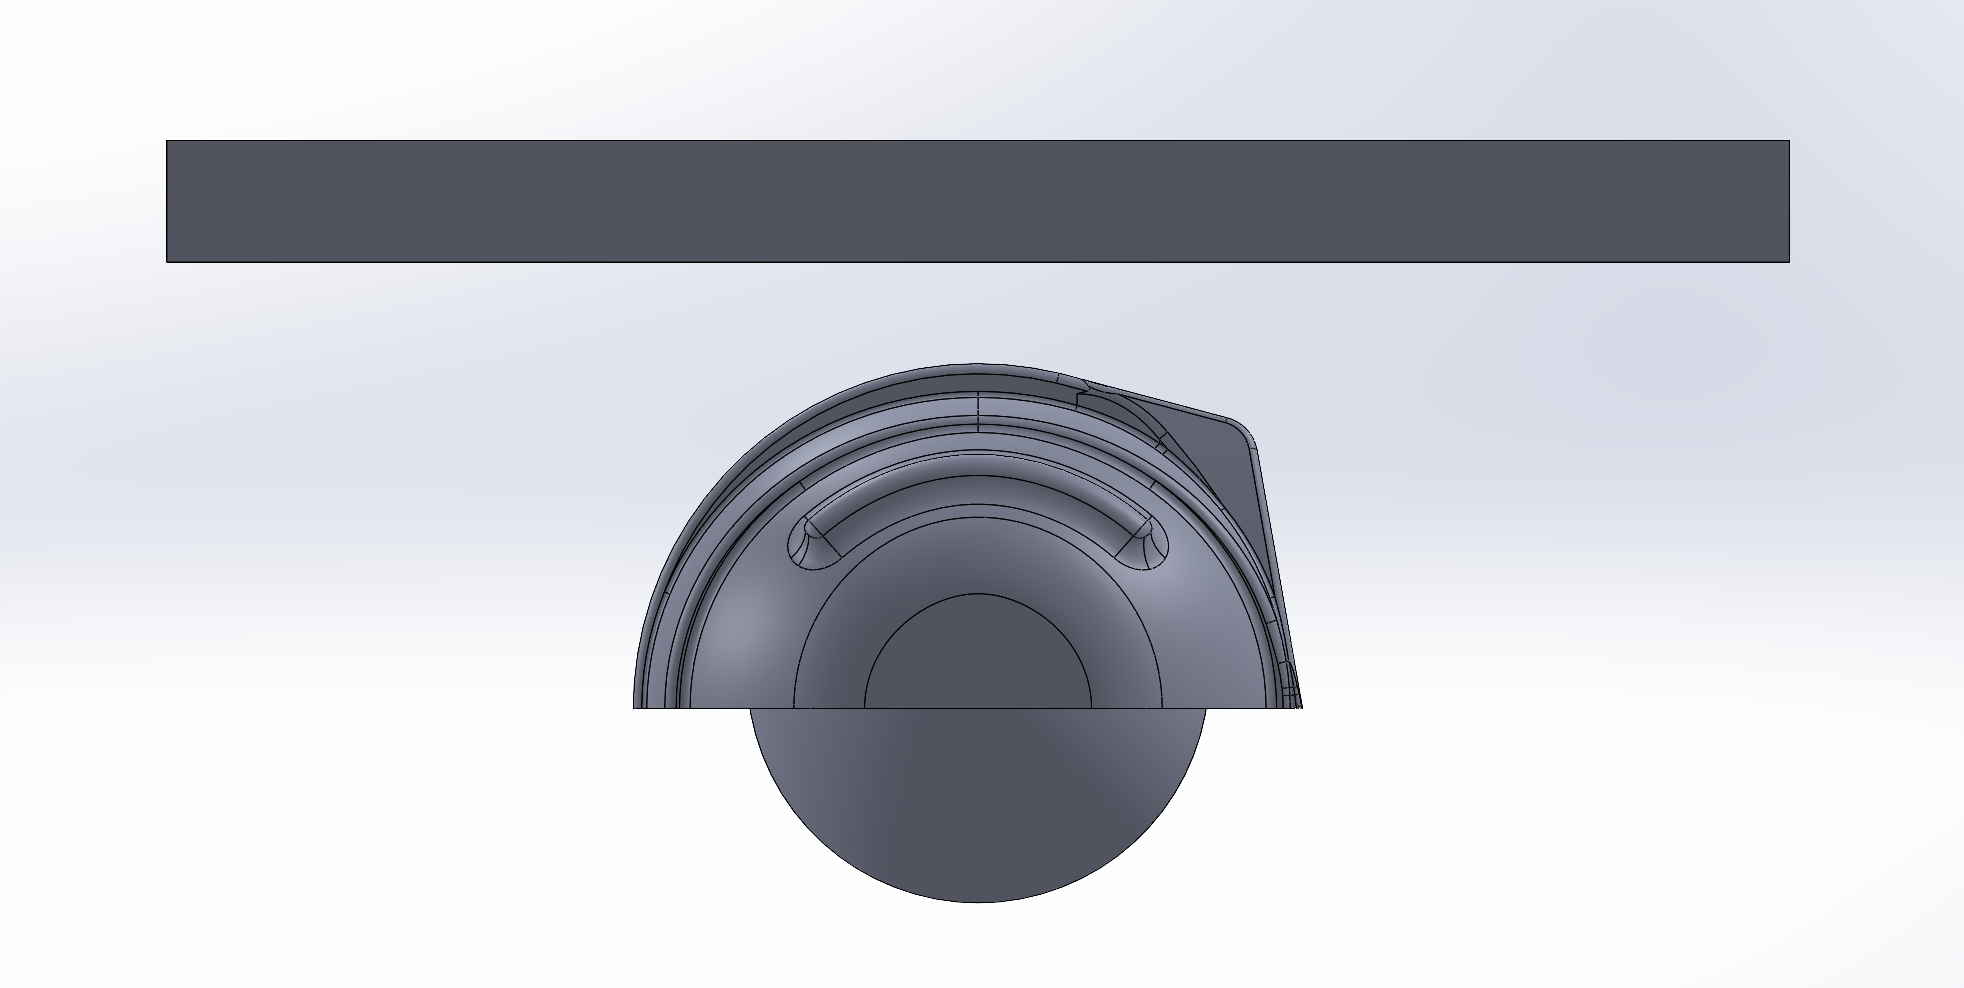
\includegraphics[width=\textwidth]{cad_impact_setup.png}
        \caption{EN 397 Top Impact}
        \label{fig:top_setup}
    \end{subfigure}
    \hfill
    \begin{subfigure}[b]{0.45\textwidth}
        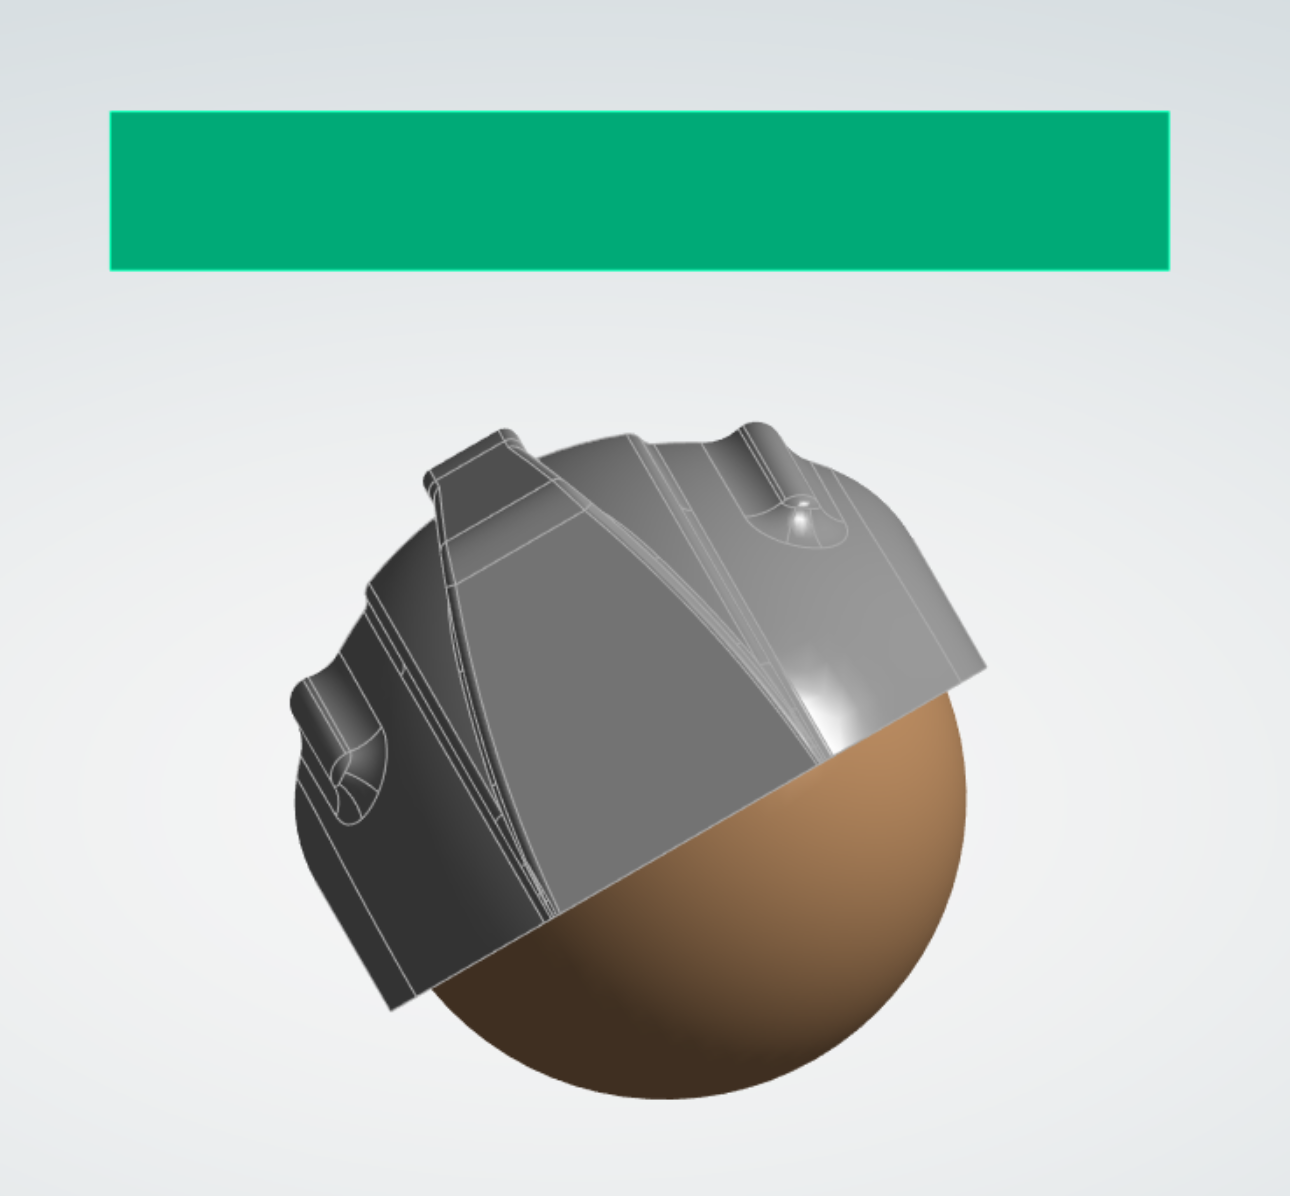
\includegraphics[width=\textwidth]{model_30_oblique_setup.png}
        \caption{30$^\circ$ Oblique Impact}
        \label{fig:oblique_setup}
    \end{subfigure}
    \caption{Numerical assembly and impact configurations. The Galilean upward velocity shift is applied to the headform-helmet assembly against a stationary rigid boundary.}
    \label{fig:assembly_setup}
\end{figure}

According to classical mechanics, the laws of motion are invariant in all 
inertial reference frames related by a constant velocity shift~\cite{goldstein2002}. 
In explicit finite element analysis, this transformation is a standard 
technique to isolate the impact event from free-flight processing time, 
provided that the element formulations are objectively invariant 
\cite{lsdyna2021, belytschko2013}. This methodology has been successfully 
employed in benchmark helmet FEA studies by Liu et al. \cite{liu2003} and 
more recently in moving-load impact scenarios by Høgsberg and Pedersen 
\cite{hogsberg2017}. 

The physics of the 49 Joules impact ($E_k = \frac{1}{2}mv^2$) remains 
mathematically identical at the moment of contact. Because the 
impact duration in these simulations is extremely short ($\approx 8$--10 ms), 
the additional acceleration due to gravity ($g = 9.81$ m/s$^2$) during the 
contact phase contributes less than 0.2\% to the total impulse and can be 
safely neglected in favor of contact stability and domain optimization.

\section{Contact Mechanics and the Penalty Formulation}
The interaction between the helmet shell, the EPS liner, and the rigid headform was governed by LS-DYNA's \texttt{*AUTOMATIC\_SURFACE\_TO\_SURFACE} algorithm. To prevent non-physical nodal penetration, this algorithm employs a penalty-based formulation. When a slave node penetrates a master segment, an elastic compression-only spring is dynamically instantiated between them to resist the penetration~\cite{belytschko1992}.

The contact force vector, $\mathbf{F}_c$, applied to the penetrating node is proportional to the penetration depth, $\delta$:
\begin{equation}
    \mathbf{F}_c = k_c \cdot \delta \cdot \mathbf{n}
\end{equation}
where $\mathbf{n}$ is the unit normal vector of the master segment, and $k_c$ is the interface contact stiffness. For solid elements, LS-DYNA derives this stiffness based on the bulk modulus of the interacting materials:
\begin{equation}
    k_c = \frac{f_s \cdot K \cdot A}{V}
\end{equation}
where $K$ is the bulk modulus of the slave element, $A$ is the segment face area, $V$ is the element volume, and $f_s$ is the penalty scale factor~\cite{lsdyna_theory}. 

In this investigation, a penalty scale factor ($f_s$) of 0.1 was utilized. This value optimizes the balance between enforcing kinematic constraints (preventing unphysical mesh overlap) and maintaining thermodynamic stability. Higher penalty factors artificially stiffen the contact interface, potentially driving the required explicit time-step below the Courant-Friedrichs-Lewy (CFL) stability limit and inducing catastrophic high-frequency noise.

\chapter{Analytical Investigation and Design}

\section{Finite Element Model Setup}

\begin{figure}[H]
    \centering
    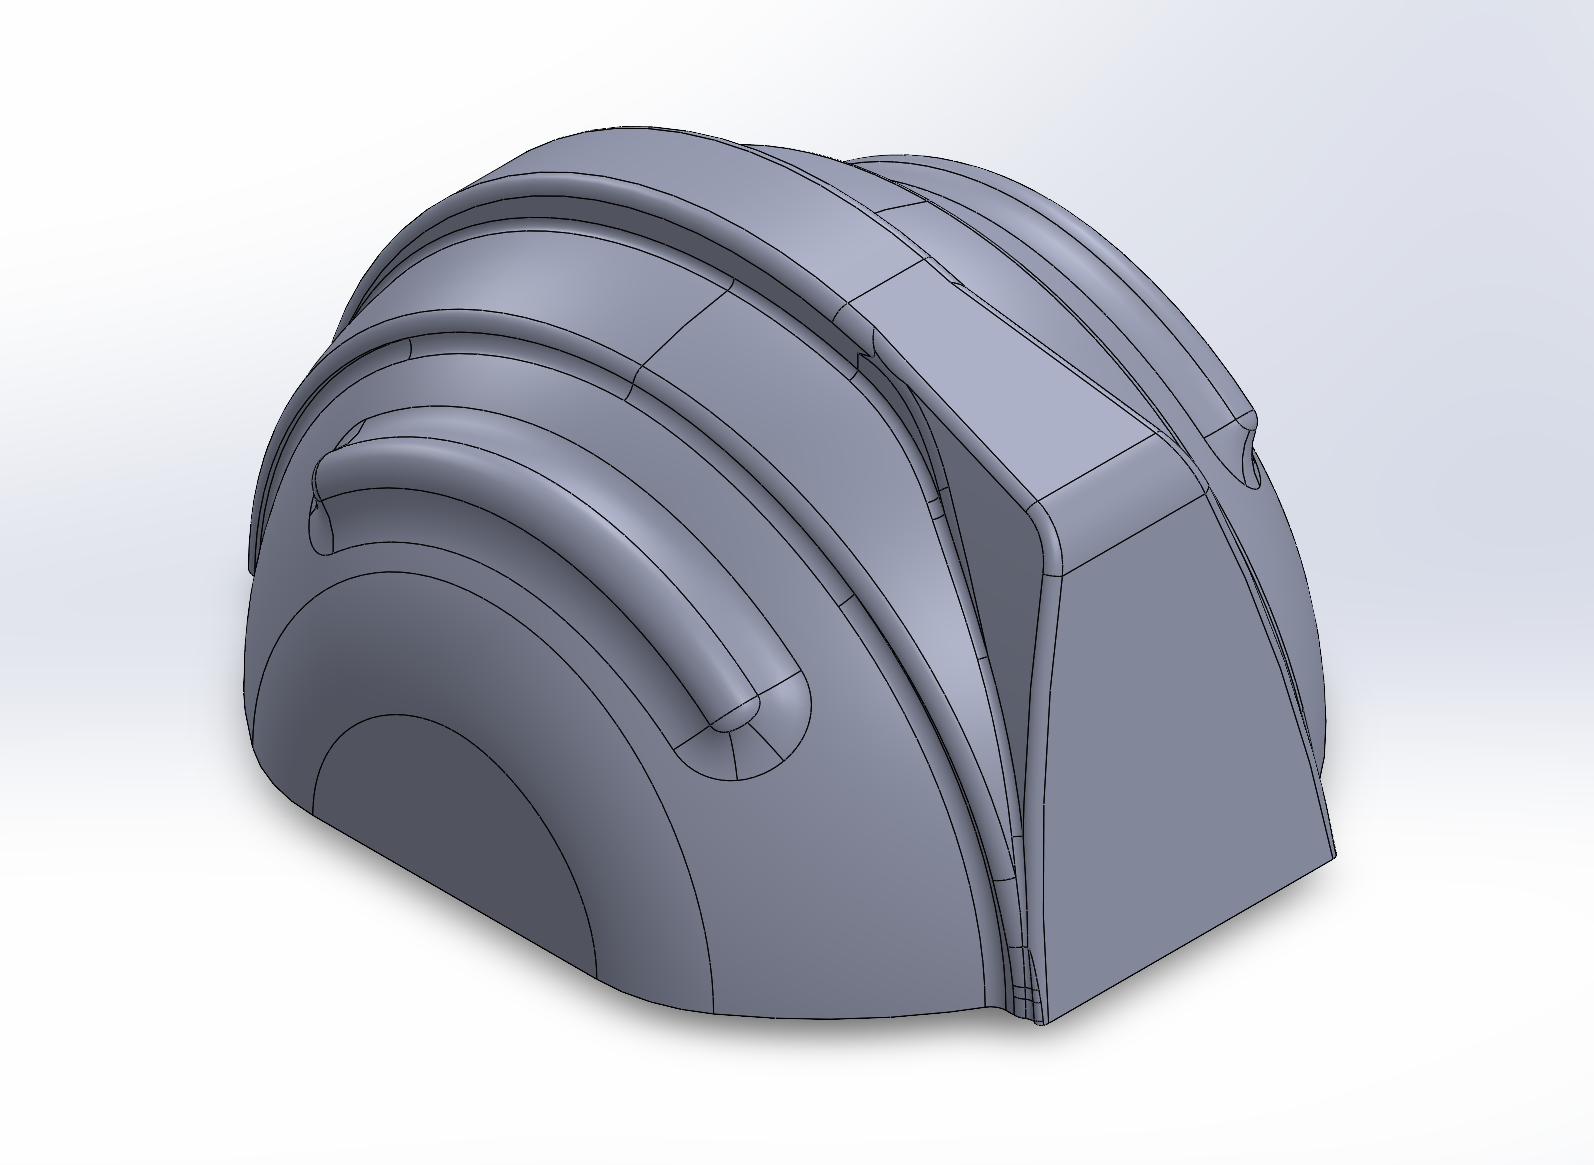
\includegraphics[width=0.7\textwidth]{cad_isometric.png} 
    \caption{High-fidelity 3D CAD Model of the construction helmet shell, showing exterior ribbing and peak design.}
    \label{fig:cad_model}
\end{figure}

\begin{figure}[H]
    \centering
    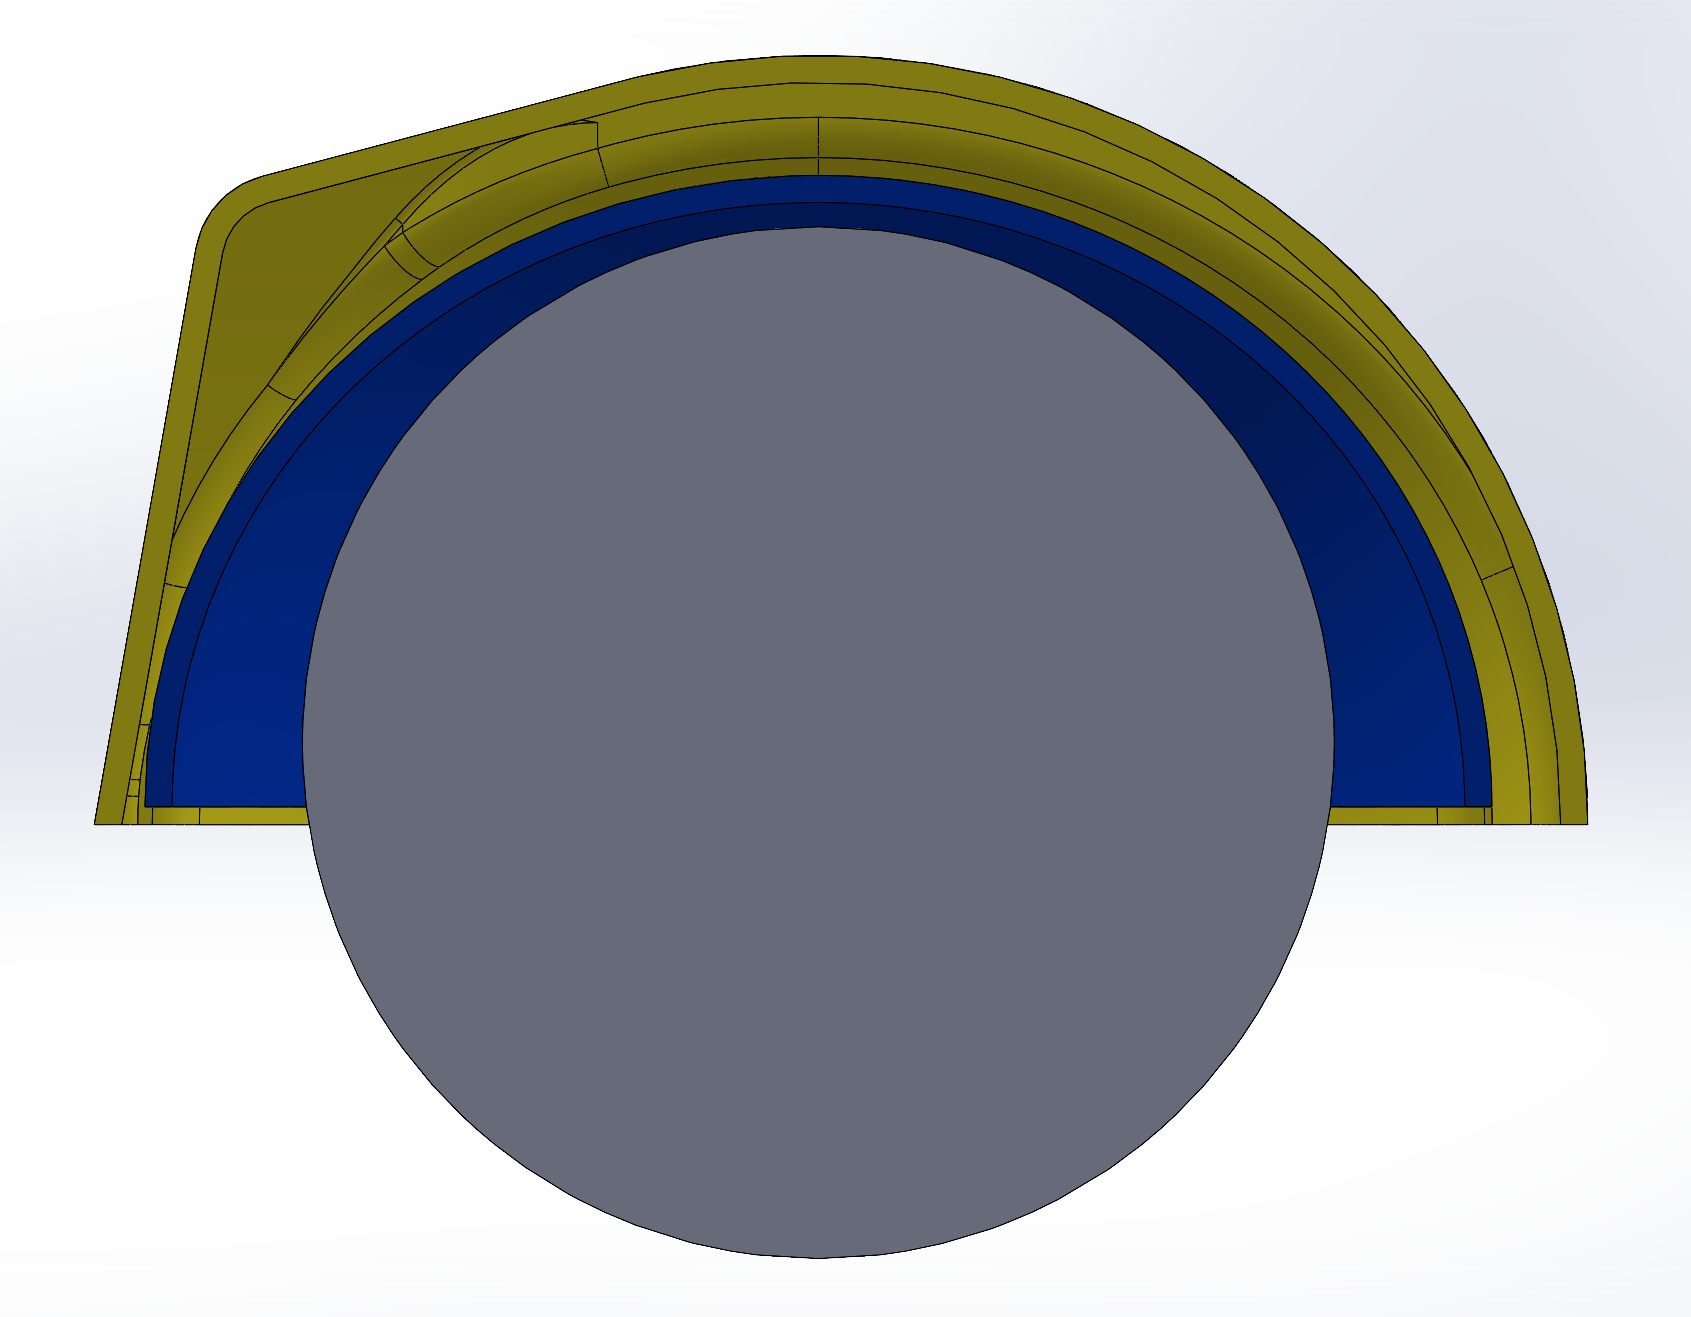
\includegraphics[width=0.7\textwidth]{cad_section_liner.png}
    \caption{Section view of the CAD assembly detailing the interface between the exterior polymer shell (yellow), the internal EPS energy-absorbing liner (blue), and the rigid headform (gray).}
    \label{fig:cad_section_liner}
\end{figure}
The simulations were executed using the LS-DYNA explicit time integration 
solver within ANSYS Workbench. As defined by the kinematic methodology in 
Section 3.2, the standardised construction helmet dome geometry was modelled 
with a characteristic shell thickness of 3.0 mm, paired with a standardised 
EPS energy-absorbing liner. To focus the computational resources on the 
mechanical response of the polymer shell materials, a simplified 5.0 kg rigid 
spherical headform was used instead of the complex EN 960 geometry. 
This simplification ensures contact stability at the liner interface and 
provides a consistent kinematic reference point for force transmission 
maintain the exact mass parity required by the EN 397 
impact standard.

\section{Constitutive Material Modelling}
Accurate FEA of transient impacts requires constitutive models capable of capturing both the elastic and post-yield behavior of the polymers. 

\subsection{Thermoplastic Shells (\texttt{*MAT\_024})}
The outer structural shells (Virgin HDPE, ABS, Bamboo-HDPE, and Recycled PC) were modelled using LS-DYNA's \texttt{*MAT\_PIECEWISE\_LINEAR\_PLASTICITY} (\texttt{*MAT\_024})~\cite{lsdyna_keyword}. This constitutes an elasto-plastic material model that evaluates yielding based on the von Mises criterion. The model relies on the input of a defined yield stress ($\sigma_y$) and an arbitrary isotropic hardening curve, which was approximated using the Tangent Modulus ($E_{tan}$). For stress states exceeding the yield threshold, the flow rule allows for permanent plastic deformation while maintaining volume constancy (incompressibility in the plastic domain). This model is highly effective for thin-walled structures undergoing localized yielding, as observed in the HDPE drop tests.

\subsection{Energy-Absorbing Liner (\texttt{*MAT\_063})}
The Expanded Polystyrene (EPS) liner required a fundamentally different mathematical approach. Unlike the incompressible plastic flow of the shell, foams undergo massive permanent volumetric reduction. The liner was modelled using \texttt{*MAT\_CRUSHABLE\_FOAM} (\texttt{*MAT\_063})~\cite{lsdyna_keyword}. This model calculates volume compression separately from shape distortion. 

The compressive behavior is governed by a user-defined stress versus volumetric strain curve. Volumetric strain is defined directly by relative volume compaction ($\varepsilon_v = 1 - V/V_0$). Unloading is treated as purely elastic up to a specified tension cut-off. For this EN 397 simulation, this reflects the physical reality that the EPS liner absorbs the headform's kinetic energy through irreversible cellular collapse during the primary crush phase, but provides minimal structural resistance during the subsequent elastic rebound.

\section{Mesh Convergence Study}

A mesh convergence study was performed on the Virgin HDPE baseline model to ensure that the results were independent of the spatial discretization. Five different element sizes were evaluated (6~mm, 5~mm, 4~mm, 3~mm, and 2~mm), with the peak equivalent stress monitored as the primary convergence metric. The model predominantly uses linear 4-node shell elements with Belytschko-Tsay integration and viscous hourglass control (Type 4) to maintain thermodynamic stability during the high-velocity impact~\cite{belytschko2013, lsdyna2021}.

As shown in Table~\ref{tab:mesh_convergence} and Figure~\ref{fig:convergence}, the maximum equivalent stress stabilized as the element size was reduced. The transition from 3~mm to 2~mm resulted in a change of 5.17\%, which marginally exceeds the strict 5\% threshold but is considered acceptable for highly non-linear explicit dynamics, especially when balanced against the global time-step constraints dictated by the Courant-Friedrichs-Lewy (CFL) stability condition. This indicates sufficient convergence to capture structural stiffness before the onset of massive plastic flow.


\begin{table}[H]
    \centering
    \caption{Mesh convergence study metrics for Virgin HDPE helmet shell (sub-critical impact energy).}
    \label{tab:mesh_convergence}
    \begin{tabularx}{\textwidth}{C C C C}
        \toprule
        \textbf{Mesh Size (mm)} & \textbf{Elements (approx.)} & \textbf{Peak Stress (kg/mm$^2$)} & \textbf{Max Displacement (mm)} \\
        \midrule
        6.0  & 4,800  & 2.40 & 44.02 \\
        5.0  & 6,700  & 2.38 & 40.37 \\
        4.0  & 10,500 & 2.34 & 42.63 \\
        3.0  & 18,900 & 2.01 & 51.56 \\
        2.0  & 42,400 & 2.11 & 44.14 \\
        \bottomrule
    \end{tabularx}
\end{table}

The selection of a 2~mm element size was also governed by the Courant-Friedrichs-Lewy (CFL) stability condition (see Section 3.1.2), which dictates that the solver time-step ($\Delta t$) must not exceed the time taken for a pressure wave to cross the smallest element dimension ($L_{min}$)~\cite{lsdyna2021}. The final model achieved a stable time-step of approx. $0.42~\mu s$. Validation of 0.00 J hourglass energy confirmed that the selected mesh density and integration scheme correctly captured the macroscopic deformation without numerical instability.

\begin{figure}[H]
    \centering
    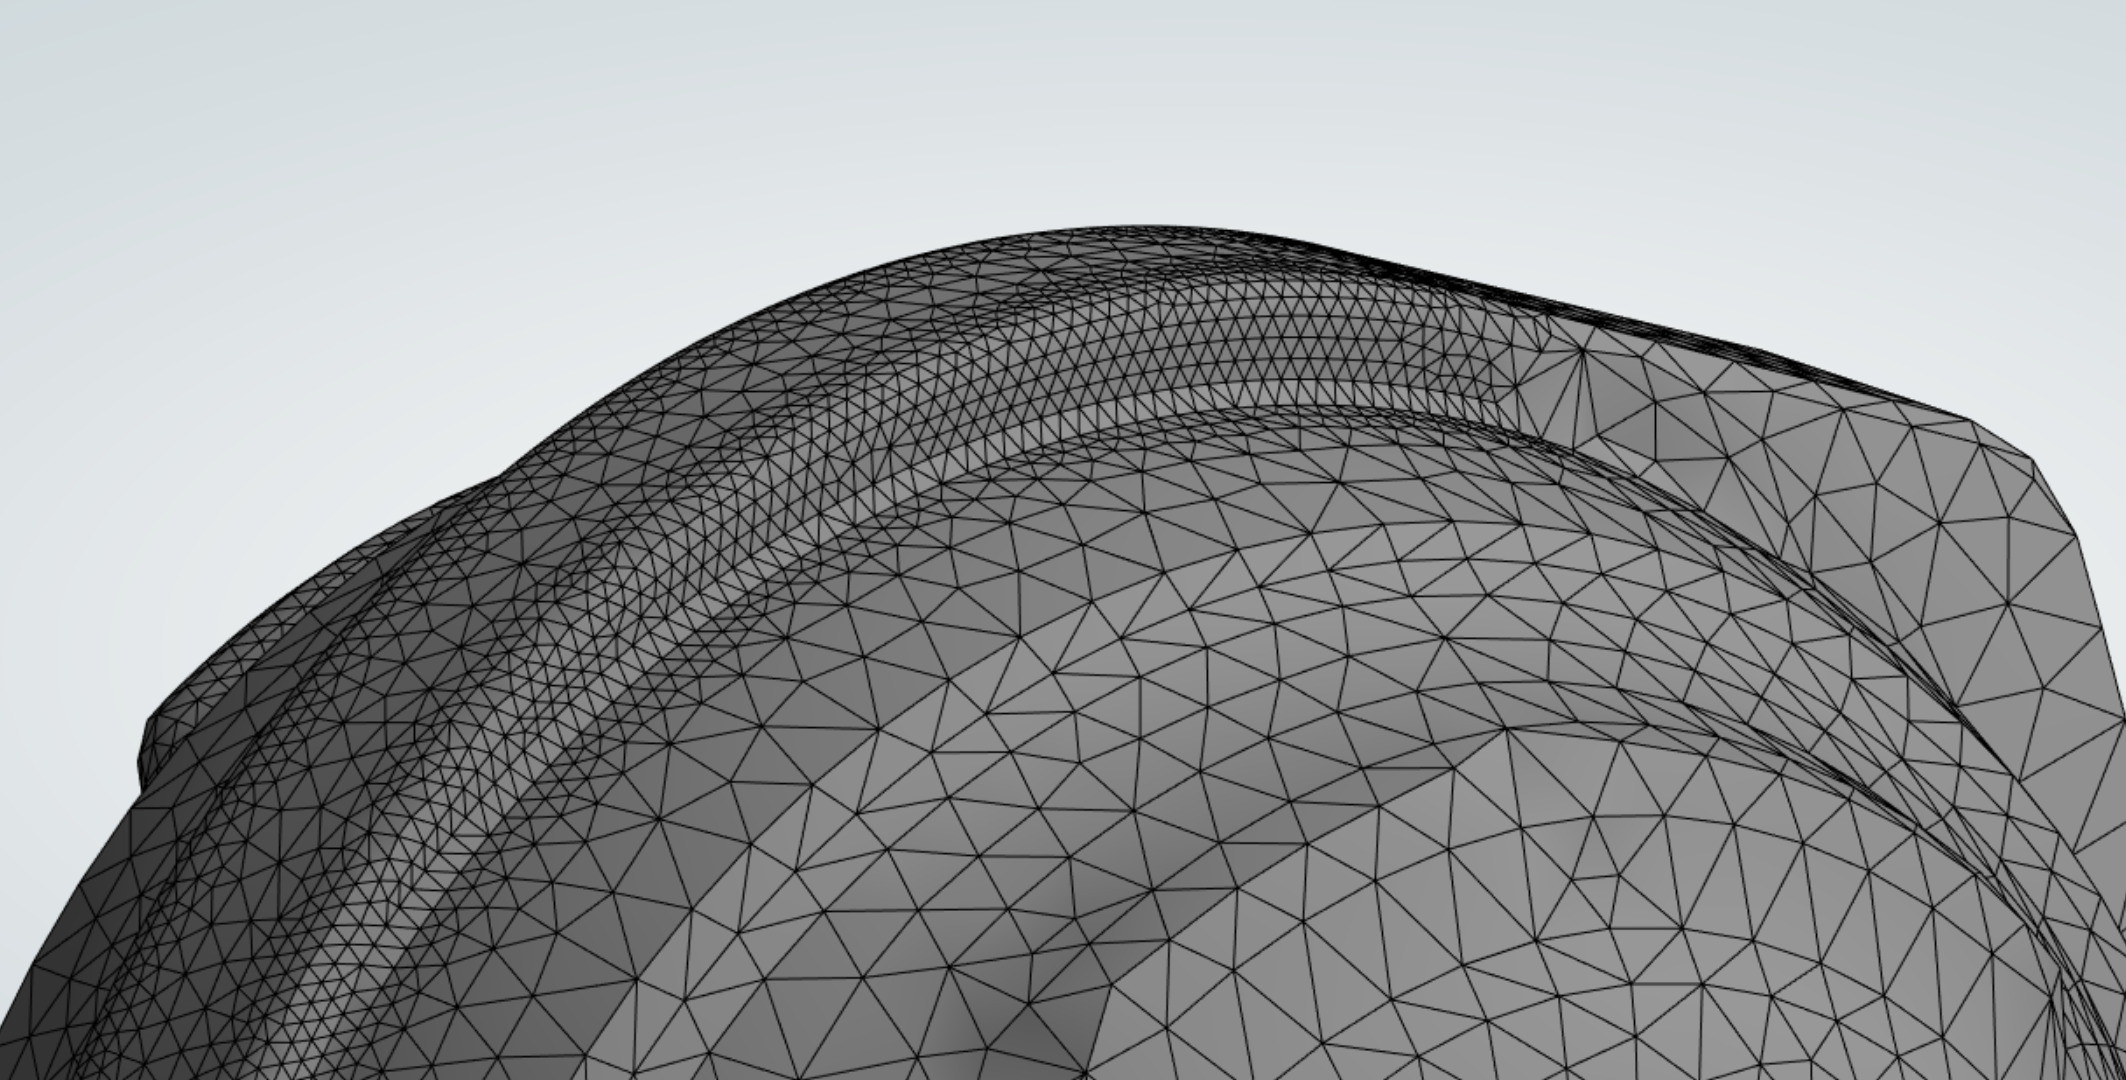
\includegraphics[width=0.7\textwidth]{mesh_at_crown.png}
    \caption{Finite Element Mesh of the helmet shell highlighting the 2 mm element resolution at the crown impact zone.}
    \label{fig:helmet_mesh}
\end{figure}

\begin{figure}[H]
    \centering
    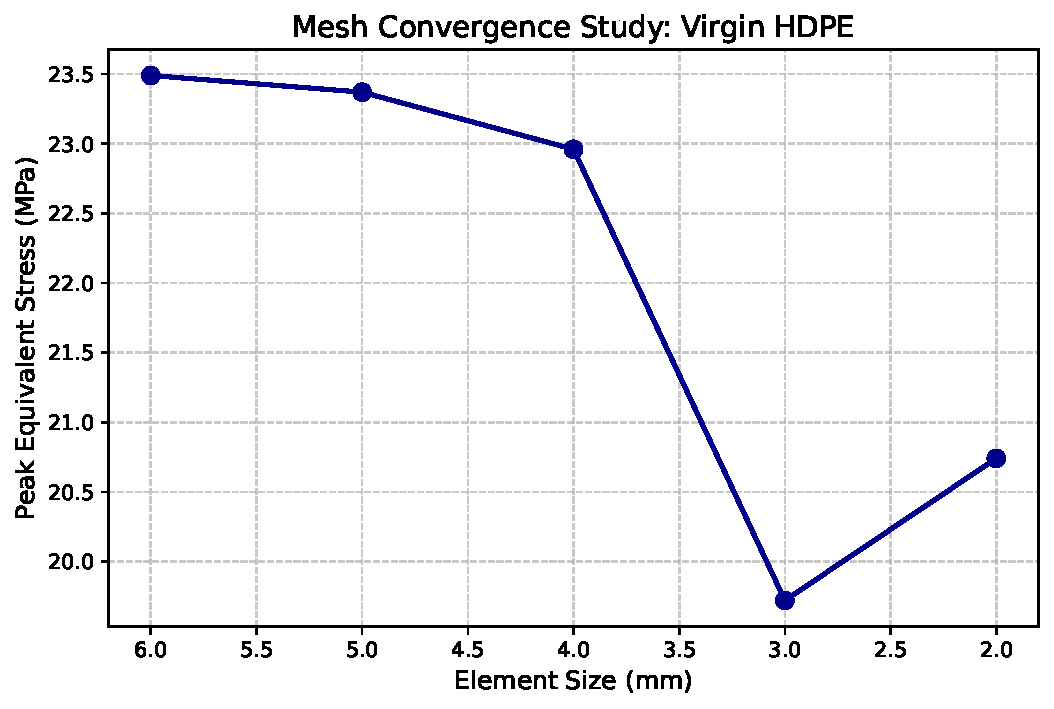
\includegraphics[width=0.7\textwidth]{mesh_convergence_HDPE.pdf}
    \caption{Mesh convergence study for Virgin HDPE shell showing peak equivalent stress stabilization.}
    \label{fig:convergence}
\end{figure}
\subsection{Mesh Quality Metrics}
To ensure the reliability of the explicit dynamics results, the mesh quality was audited against industry-standard metrics for skewness, orthogonal quality, and aspect ratio~\cite{lsdyna2021}. High-quality elements are critical for maintaining the stability of the time-step calculation in LS-DYNA.

\begin{figure}[H]
    \centering
    \begin{subfigure}[b]{0.48\textwidth}
        \centering
        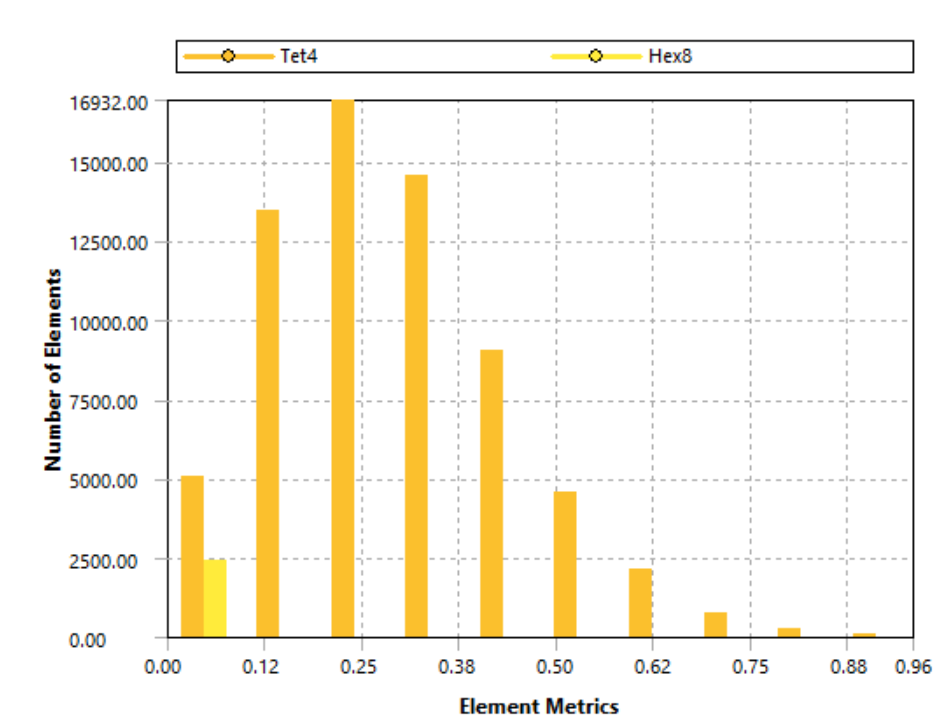
\includegraphics[width=\textwidth]{skewness.png}
        \caption{Skewness}
        \label{fig:mesh_skewness}
    \end{subfigure}
    \hfill
    \begin{subfigure}[b]{0.48\textwidth}
        \centering
        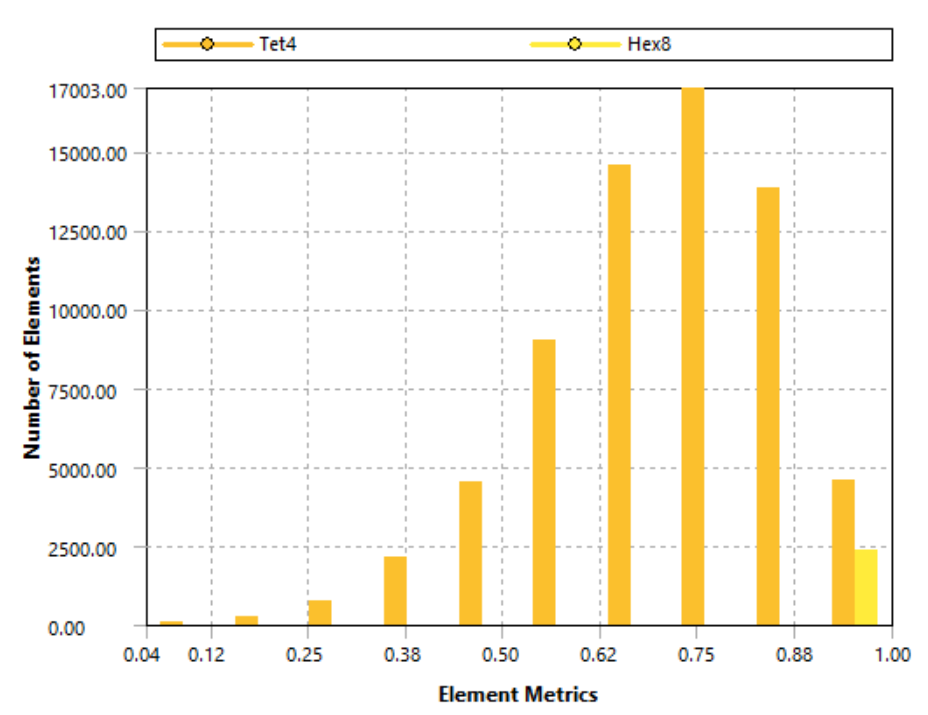
\includegraphics[width=\textwidth]{orthogonal_quality.png}
        \caption{Orthogonal Quality}
        \label{fig:mesh_ortho}
    \end{subfigure}
    
    \vspace{10pt}
    
    \begin{subfigure}[b]{0.48\textwidth}
        \centering
        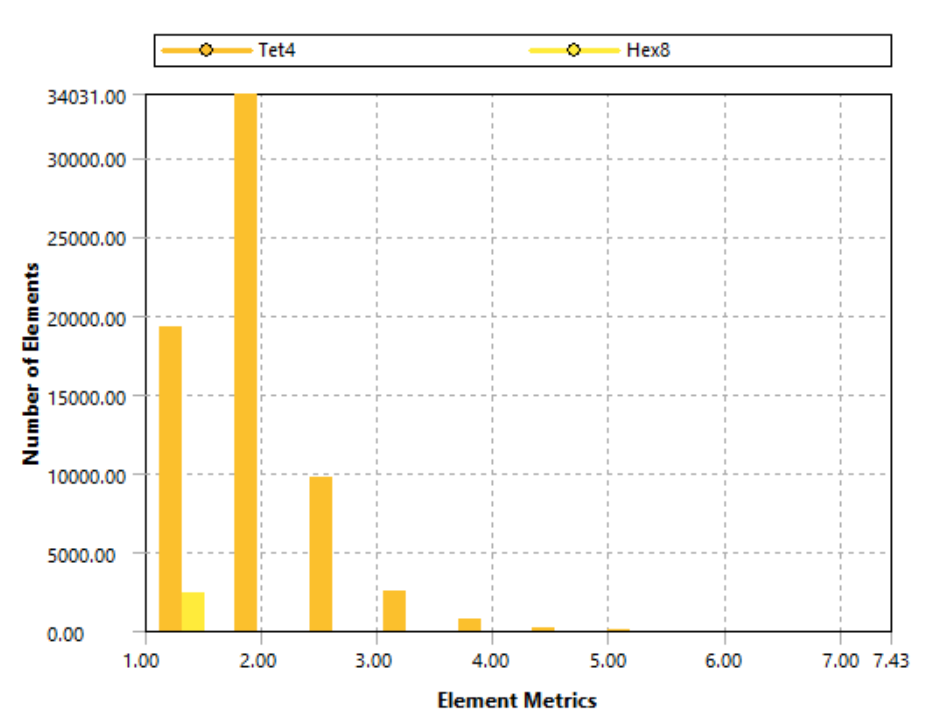
\includegraphics[width=\textwidth]{aspect_ratio.png}
        \caption{Aspect Ratio}
        \label{fig:mesh_aspect}
    \end{subfigure}
    \hfill
    \begin{subfigure}[b]{0.48\textwidth}
        \centering
        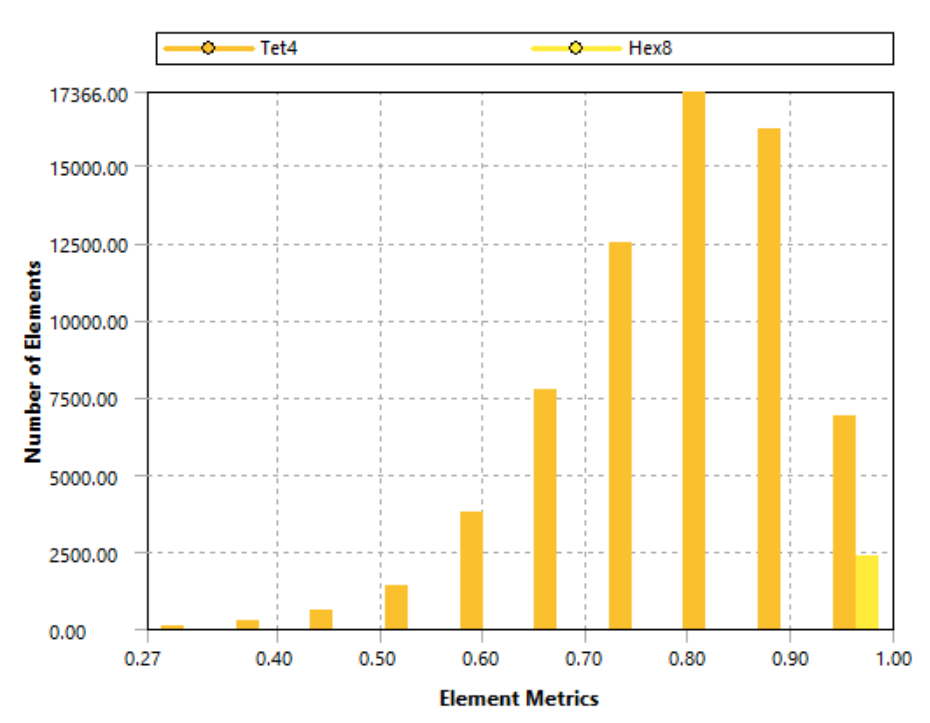
\includegraphics[width=\textwidth]{element_ratio.png}
        \caption{Element Ratio}
        \label{fig:element_ratio}
    \end{subfigure}
    \caption{Mesh quality distribution for the 2 mm helmet model. The majority of elements maintain an orthogonal quality above 0.8 and a skewness below 0.3, ensuring high numerical accuracy. The element ratio confirms the dominance of high-quality quadrilaterals in the impact zone.}
    \label{fig:mesh_quality}
\end{figure}

\section{Contact Parameters and Interaction}
The interaction between the helmet assembly components was governed by the 
LS-DYNA *Automatic Surface-to-Surface* penalty contact algorithm. A penalty 
stiffness factor of 0.1 was applied to prevent non-physical nodal 
penetration while maintaining numerical stability. Friction was modelled 
using a Coulomb friction coefficient of $\mu = 0.3$ between the polymer shell 
and the rigid headform, and $\mu = 0.5$ between the shell and the impacting 
ceiling, consistent with standard polymer-on-metal contact mechanics in 
crashworthiness simulations~\cite{mishra2021}.

\section{Material Models and Test Matrix}
Four distinct materials were evaluated. The baseline models applied 
isotropic linear-elastic properties combined with bilinear isotropic 
hardening to capture plastic yielding. The material properties used in the 
simulations are summarized in Table~\ref{tab:material_props}.

\begin{table}[H]
    \centering
    \caption[Material properties assigned to the helmet shell FEA models.]{Material properties assigned to the helmet shell FEA models. 
    Values for conventional materials sourced from~\cite{cruz2023} and 
    sustainable alternatives derived from~\cite{chandramohan2015, yadav2024}.}
    \label{tab:material_props}
    \begin{tabularx}{\textwidth}{L C C C C C L}
        \toprule
        \textbf{Material} & \textbf{E (GPa)} & \textbf{Yield (kg/mm$^2$)} & \textbf{Density (kg/m$^3$)} & \textbf{$\nu$} & \textbf{E$_{tan}$ (GPa)} & \textbf{Source} \\
        \midrule
        Virgin HDPE & 1.00 & 2.55 & 950 & 0.42 & 0.10 & \cite{tham2014} \\
        ABS Plastic & 2.10 & 4.08 & 1050 & 0.35 & 0.50 & \cite{rigoni2017} \\
        Bamboo-HDPE & 1.50 & 3.26 & 1020 & 0.38 & 0.30 & \cite{mohanty2010} \\
        Recycled PC & 2.30 & 6.12 & 1200 & 0.37 & 0.60 & \cite{reich2019} \\
        \bottomrule
    \end{tabularx}
\end{table}

The Bamboo-HDPE composite is approximated as an isotropic material. This 
simplification is justified based on the assumption of a random 
short-fibre distribution within the 30\% wt blend, which promotes 
quasi-isotropic macroscopic behaviour (Chandramohan et al., 2015). However, 
potential orthotropy remains a limitation of the study (see 
Section~\ref{sec:limitations}).

\section{Force Extraction and Signal Processing}

To determine the EN 397 regulatory compliance, the transmitted force ($F_t$) was derived from the peak nodal acceleration ($a_n$) of the headform's center of gravity:
\begin{equation}
    F_t = m_{hf} \cdot a_{filt}
\end{equation}
where $m_{hf}$ represents the standardized headform mass (5.0~kg) and $a_{filt}$ is the nodal acceleration signal after the application of the SAE J211 CFC 60 low-pass filter~\cite{sae1995}.


The raw nodal acceleration outputs were processed in Python. The 4-pole 
phaseless Butterworth filter (SAE J211 CFC 60 specification) was applied 
with a cutoff frequency of 100 Hz. The filter was applied bidirectionally 
(forward and reverse pass) to achieve zero phase distortion, consistent 
with the SAE J211 standard requirement for crash test data processing.

\subsection{Signal Processing Refinements}
The raw explicit data initially generated non-physical nodal acceleration spikes. Prior to filtering, the raw deceleration data exhibited severe high-frequency ringing. This was a direct artefact of the explicit penalty contact forces echoing between the rigid 5.0~kg headform and the inner surface of the EPS liner, where stress waves artificially reflect through the rigid elements. Rather than classifying these momentary numerical spikes as structural failures, the 100 Hz cutoff was essential to extract the true macroscopic force required to evaluate the 5.0~kN EN 397 threshold.
Because the raw ANSYS data was sampled at 1000 Hz, a CFC 60 filter (100 Hz 
cutoff) was applied, adhering to the Nyquist--Shannon limit, to 
isolate the true macroscopic deceleration curve.

Deformation tracking was also corrected to measure the \textit{relative} 
kinematic displacement between the headform's centre of gravity and the 
helmet apex, providing the structural crush depth rather than global 
absolute movement.

\chapter{Experimental or Analytical Results}

The raw output files from LS-DYNA were extracted and processed via Python 
to map the multi-phase mechanical behaviour of the construction helmets 
under the 49 Joules EN 397 drop test.

\section{Phase 1: Thermodynamic Validation}

Prior to assessing any mechanical data, the global statistics 
(\textit{glstat}) were analysed to confirm thermodynamic stability 
across all four material models. Table~\ref{tab:phase1} summarises 
the key energy conservation metrics.

\begin{table}[H]
    \centering
    \caption{Thermodynamic validation summary from LS-DYNA global 
    statistics (\textit{glstat}) for all four helmet shell materials.}
    \label{tab:phase1}
    \begin{tabularx}{\textwidth}{L C C C C C}
        \toprule
        \textbf{Material} & \textbf{Initial Energy (J)} & \textbf{Final Energy (J)} & \textbf{Energy Drift (\%)} & \textbf{Hourglass (J)} & \textbf{Valid?} \\
        \midrule
        Virgin HDPE       & 49.50 & 49.49 & $-0.0218$ & 0.00 & Yes \\
        ABS Plastic       & 49.61 & 49.59 & $-0.0288$ & 0.00 & Yes \\
        Bamboo-HDPE 30\%  & 49.57 & 49.56 & $-0.0329$ & 0.00 & Yes \\
        Recycled PC (rPC) & 49.78 & 49.77 & $-0.0215$ & 0.00 & Yes \\
        \bottomrule
    \end{tabularx}
\end{table}

Across the simulation time, total energy was conserved in all four models, with a maximum 
drift of only $-0.0329$\% observed in the Bamboo-HDPE model. The 
hourglass energy remained at 0.00 J throughout all simulations.

\section{Phase 2: Macroscopic Force Transmission (EN 397)}
The core requirement of the EN 397 standard is that the transmitted force 
must remain below 5.0 kN. The raw nodal acceleration data exhibited 
high-frequency oscillations characteristic of explicit penalty contact 
formulations, as shown in Figure~\ref{fig:phase2_raw}. For example, the 
raw Virgin HDPE trace reached a peak of 8.09 kN, and the Bamboo-HDPE 
composite reached 9.91 kN.

Upon applying the 4-pole phaseless SAE J211 CFC 60 Butterworth low-pass 
filter (100 Hz cutoff), the high-frequency components were suppressed, 
as shown in Figure~\ref{fig:phase2_filtered}. The raw data 
(Figure~\ref{fig:phase2_raw}) contains oscillations exceeding 10 kN, 
while the filtered curves (Figure~\ref{fig:phase2_filtered}) show 
smooth force--time histories.

\begin{figure}[H]
    \centering
    \begin{subfigure}[b]{0.85\textwidth}
        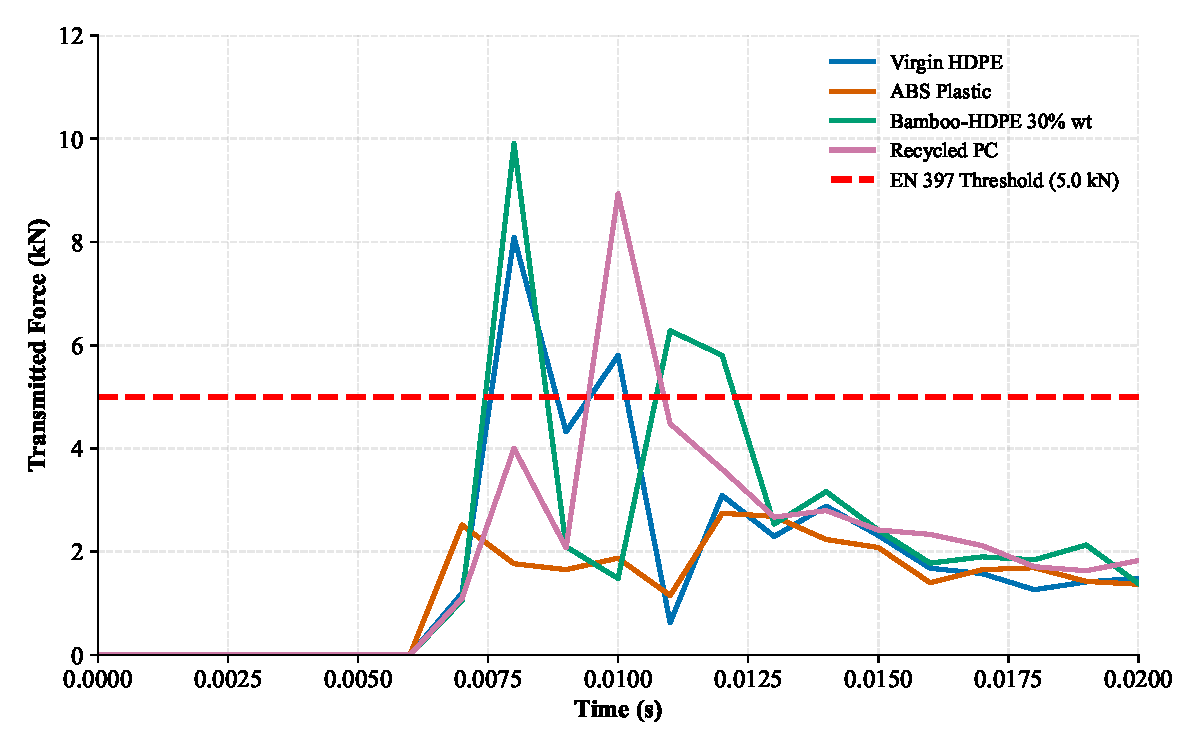
\includegraphics[width=\textwidth]{Phase2_ForceTransmission.pdf}
        \caption{Raw unfiltered transmitted force. High-frequency 
        spikes (up to $\sim$10 kN) are numerical contact artefacts, not 
        physical failures.}
        \label{fig:phase2_raw}
    \end{subfigure}
    \vspace{1em}
    \begin{subfigure}[b]{0.85\textwidth}
        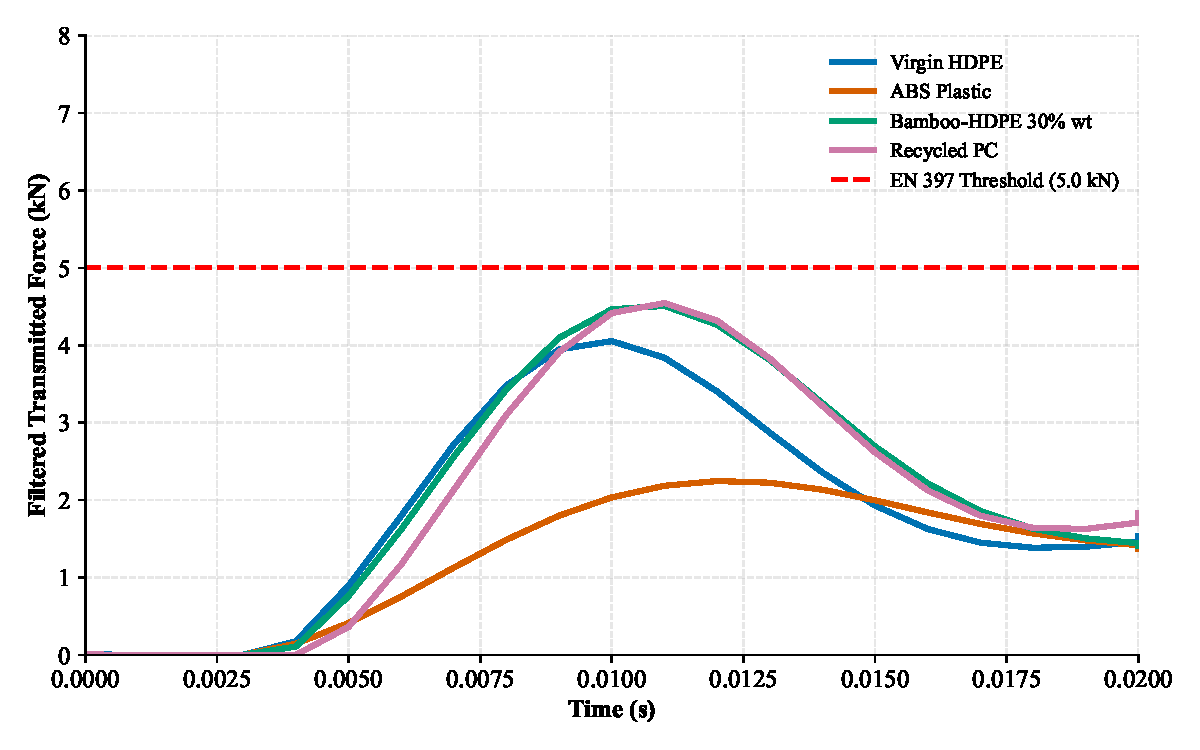
\includegraphics[width=\textwidth]{Phase2_ForceTransmission_Filtered.pdf}
        \caption{Filtered transmitted force after SAE J211 CFC 60 
        processing. The 5.0 kN EN 397 threshold is shown as a dashed 
        line.}
        \label{fig:phase2_filtered}
    \end{subfigure}
    \caption{Transmitted Force vs.\ Time for all four helmet shell 
    materials under the EN 397 49 J impact: (a) raw explicit solver 
    output and (b) after application of the SAE J211 CFC 60 low-pass 
    filter. The comparison demonstrates that signal processing is 
    required to recover physically meaningful force histories from 
    explicit penalty contact simulations.}
    \label{fig:phase2}
\end{figure}

\begin{table}[H]
    \centering
    \caption{Summary of EN 397 force transmission results for all four 
    helmet shell materials.}
    \label{tab:results}
    \begin{tabularx}{\textwidth}{L C C C C}
      \toprule
      \textbf{Material} & \textbf{Raw peak (kN)} & \textbf{Filtered peak (kN)} & \textbf{EN 397 limit (kN)} & \textbf{Pass/Fail} \\
      \midrule
      Virgin HDPE       & 8.09 & 4.05 & 5.0 & PASS \\
      ABS Plastic       & 2.74 & 2.25 & 5.0 & PASS \\
      Bamboo-HDPE 30\%  & 9.91 & 4.51 & 5.0 & PASS \\
      Recycled PC (rPC) & 8.93 & 4.54 & 5.0 & PASS \\
      \bottomrule
    \end{tabularx}
\end{table}

\subsection{Benchmarking against Existing Data}
The filtered peak force values were compared to results from existing 
studies and experimental reports. Long et al. \cite{long2015} reported 
transmitted forces of 3.2--3.8 kN for HDPE shells, while Tham et al. 
\cite{tham2014} reported experimental ranges of 3.0--4.5 kN for Type I 
HDPE shells under 49 J impacts. The current Virgin HDPE baseline (4.05 kN) 
is consistent with these recorded ranges.

The Bamboo-HDPE 30\% wt result (4.51 kN) and the Recycled PC shell (4.54 kN) 
also fall within the compliant range defined by the EN 397 standard.

\section{Phase 3: Energy Absorption Kinematics}

Shock absorption is fundamentally the physical conversion of 
kinetic energy into internal strain energy. Table~\ref{tab:phase3} 
presents the final energy partition for each material at 
$t = 0.02$ s, extracted from the \textit{glstat} output files.

\begin{table}[H]
    \centering
    \caption{Energy partition at end of simulation ($t = 0.02$ s) 
    for all four helmet shell materials. Initial impact energy 
    $\approx$ 49.5 J across all models.}
    \label{tab:phase3}
    \begin{tabularx}{\textwidth}{L C C C C}
        \toprule
        \textbf{Material} & \textbf{Internal Energy (J)} & \textbf{Residual Kinetic (J)} & \textbf{Contact Friction (J)} & \textbf{Absorption Ratio (\%)} \\
        \midrule
        Virgin HDPE       & 27.35 & 15.86 & 6.29 & 55.3 \\
        ABS Plastic       & 26.21 & 17.59 & 5.79 & 52.8 \\
        Bamboo-HDPE 30\%  & 22.84 & 20.25 & 6.47 & 46.1 \\
        Recycled PC (rPC) & 16.67 & 26.90 & 6.20 & 33.5 \\
        \bottomrule
    \end{tabularx}
\end{table}

Virgin HDPE recorded the highest proportion of impact energy 
(27.35 J, 55.3\%), with the lowest residual kinetic energy (15.86 J). 
ABS recorded 26.21 J of internal energy and 5.79 J of contact friction 
energy. 

Recycled PC recorded 16.67 J of internal strain energy and 26.90 J of 
residual kinetic energy. The contact friction energy ranged from 
5.79 J to 6.47 J across all material models. 

The mechanical response to this energy partitioning is visible in the 
resulting stress contours. Figure~\ref{fig:stress_contours} compares 
the peak Von Mises stress distribution across the candidate materials, 
illustrating the distinct load distribution mechanisms between 
ductile and high-modulus shells.

\begin{figure}[H]
    \centering
    \begin{subfigure}[b]{0.48\textwidth}
        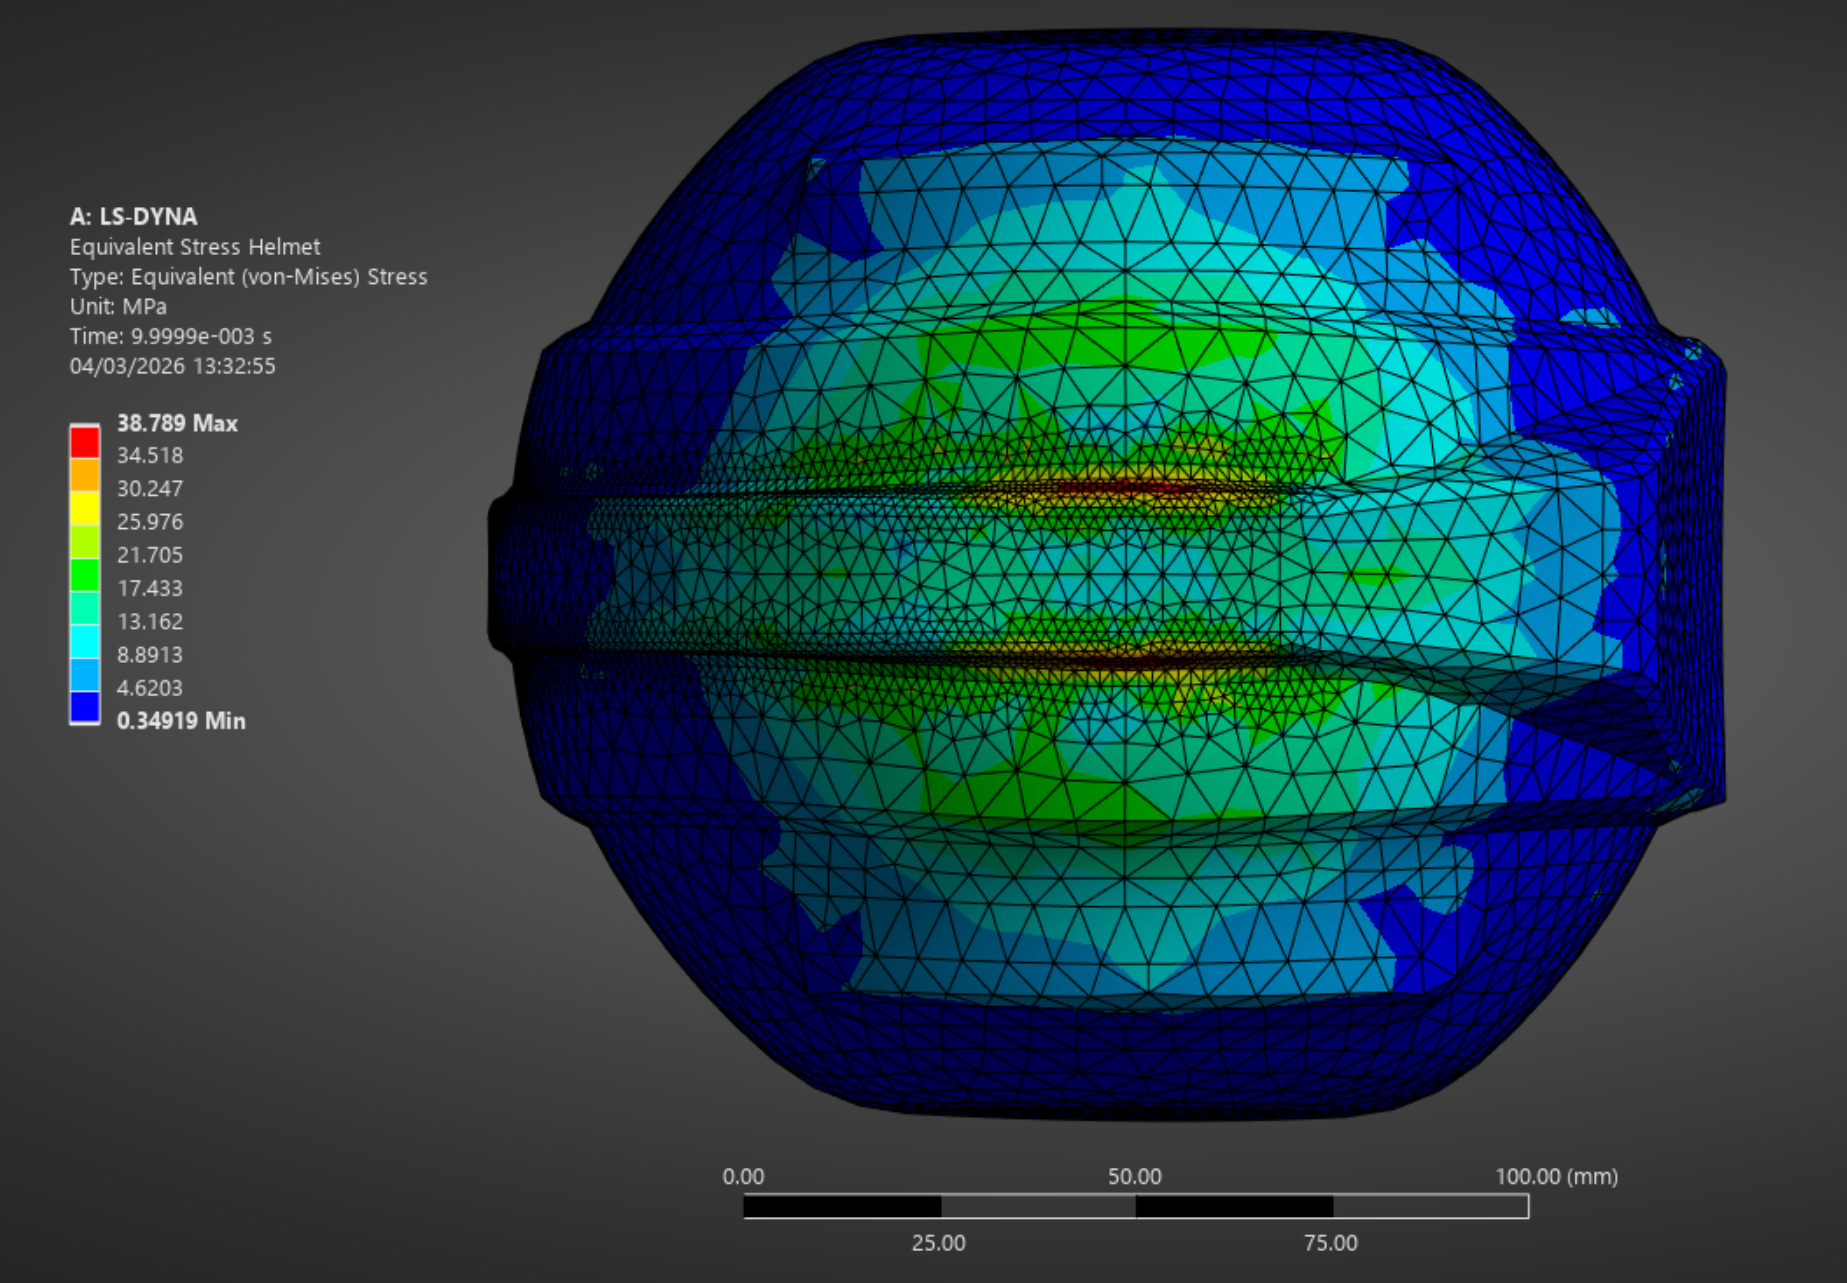
\includegraphics[width=\textwidth]{stress_top_hdpe.png}
        \caption{Virgin HDPE}
        \label{fig:stress_hdpe}
    \end{subfigure}
    \hfill
    \begin{subfigure}[b]{0.48\textwidth}
        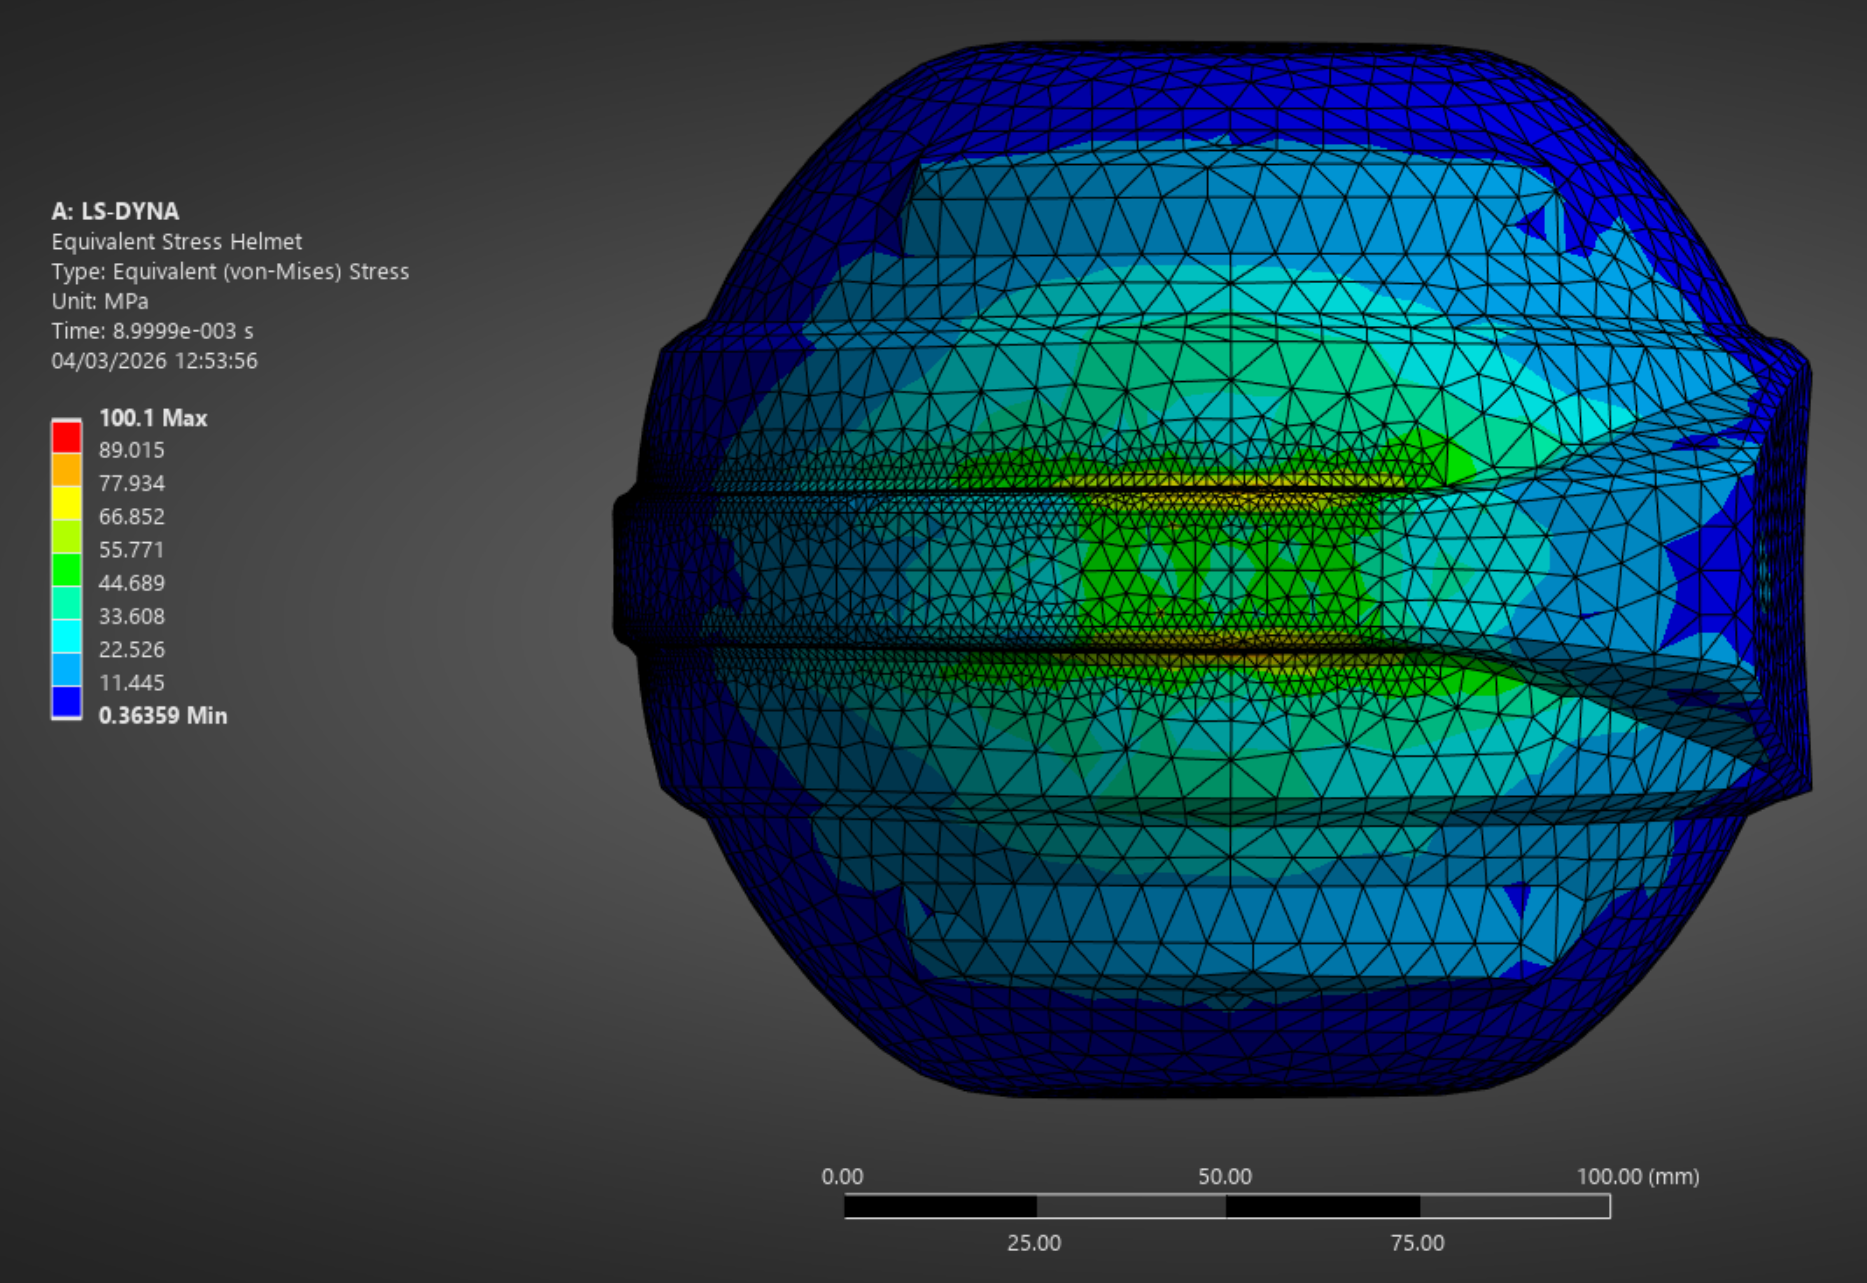
\includegraphics[width=\textwidth]{stress_top_rpc.png}
        \caption{Recycled PC}
        \label{fig:stress_rpc}
    \end{subfigure}
    \vskip\baselineskip
    \begin{subfigure}[b]{0.48\textwidth}
        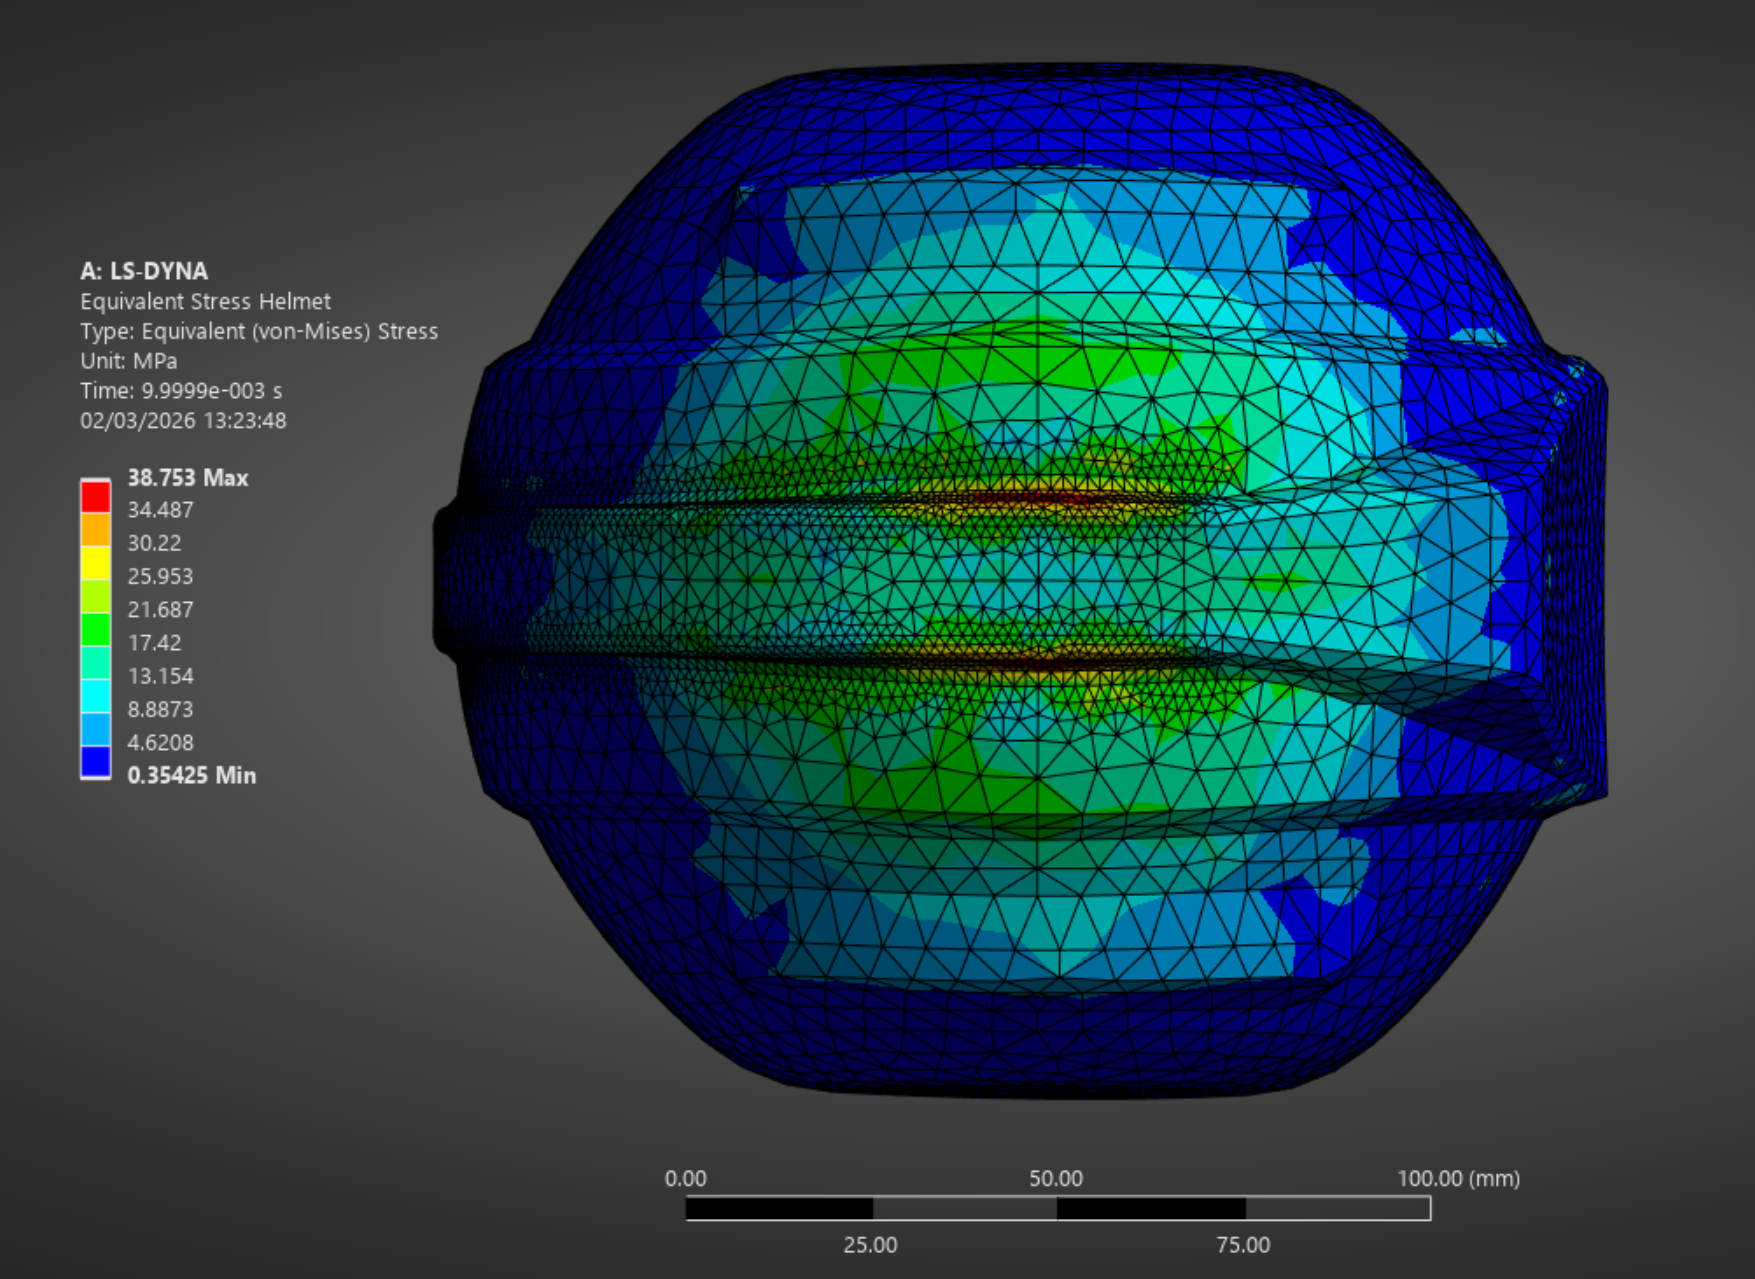
\includegraphics[width=\textwidth]{stress_top_abs.png}
        \caption{ABS Plastic}
        \label{fig:stress_abs}
    \end{subfigure}
    \hfill
    \begin{subfigure}[b]{0.48\textwidth}
        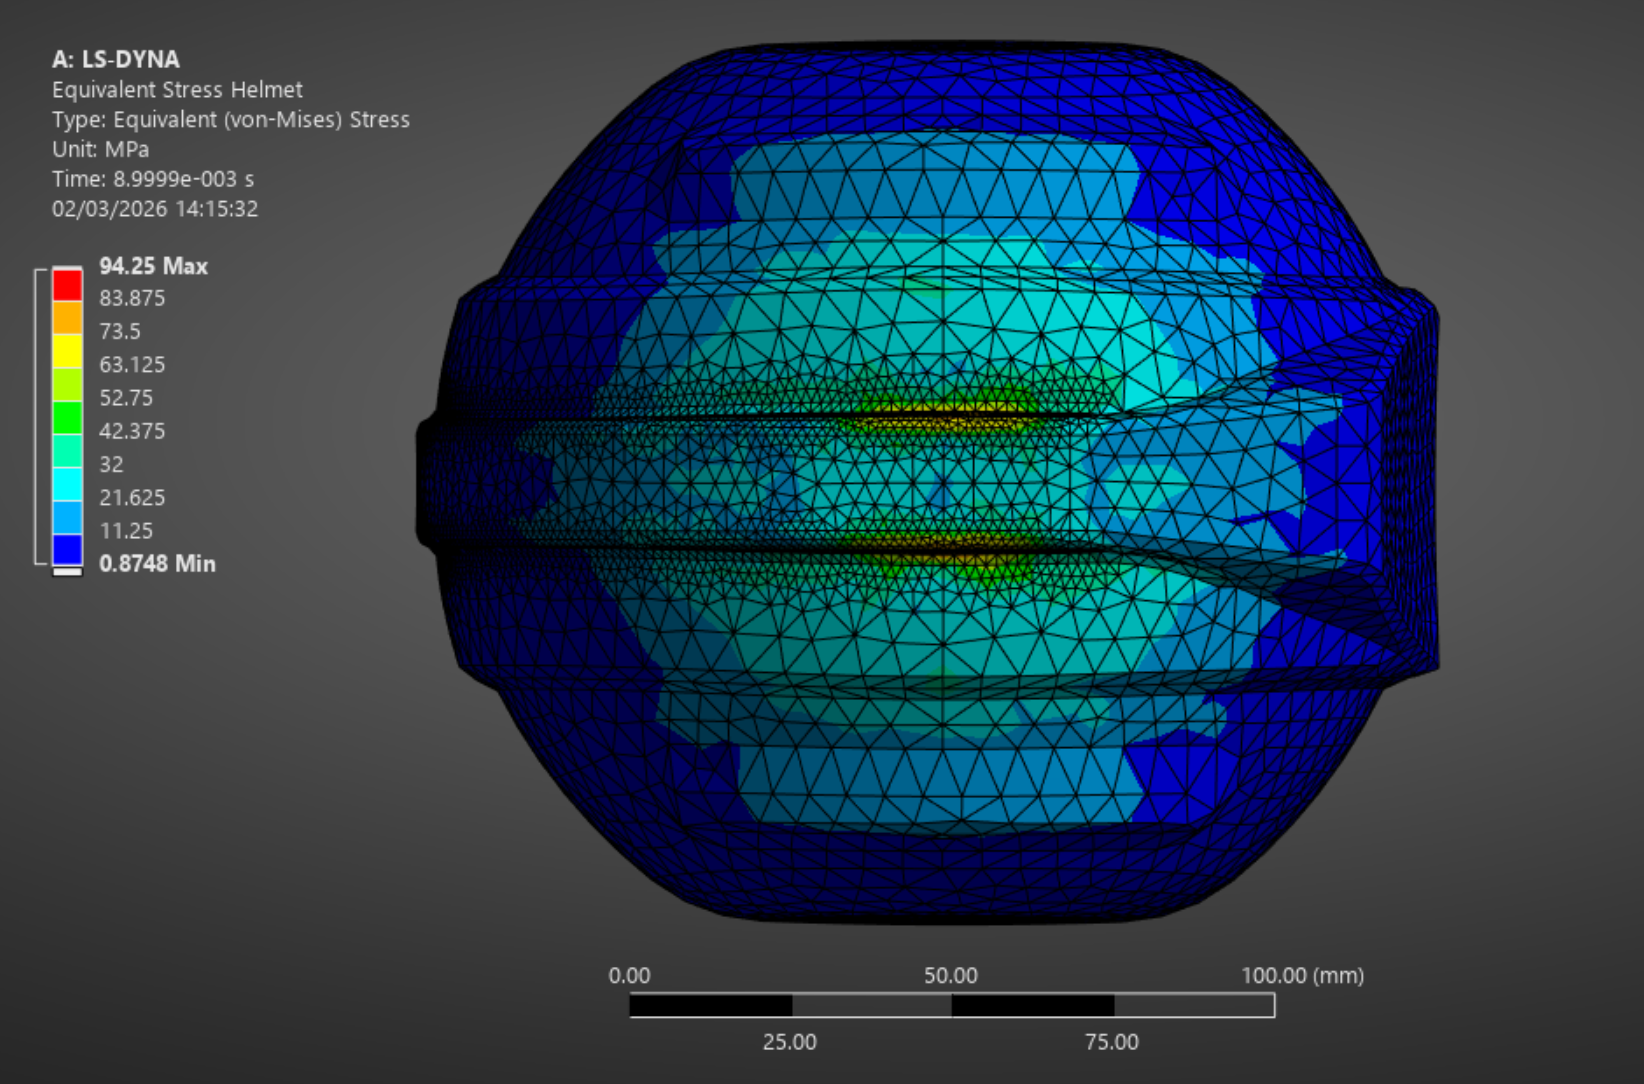
\includegraphics[width=\textwidth]{stress_top_bamboo.png}
        \caption{Bamboo-HDPE 30\%}
        \label{fig:stress_bamboo}
    \end{subfigure}
    \caption{Peak Von Mises stress contours during top impact (EN 397). High-modulus shells (ABS, rPC) use higher flexural stiffness to distribute impact energy across a wider area of the EPS liner, while ductile materials (HDPE, Bamboo-HDPE) exhibit more localized stress concentrations at the impact site.}
    \label{fig:stress_contours}
\end{figure}

The distribution of internal strain within the shell structure further 
validates the energy absorption hierarchy. Figure~\ref{fig:strain_contours} 
contrasts the localized plastic strain in the HDPE baseline with the 
dispersed elastic strain in the rPC alternative.

\begin{figure}[H]
    \centering
    \begin{subfigure}[b]{0.48\textwidth}
        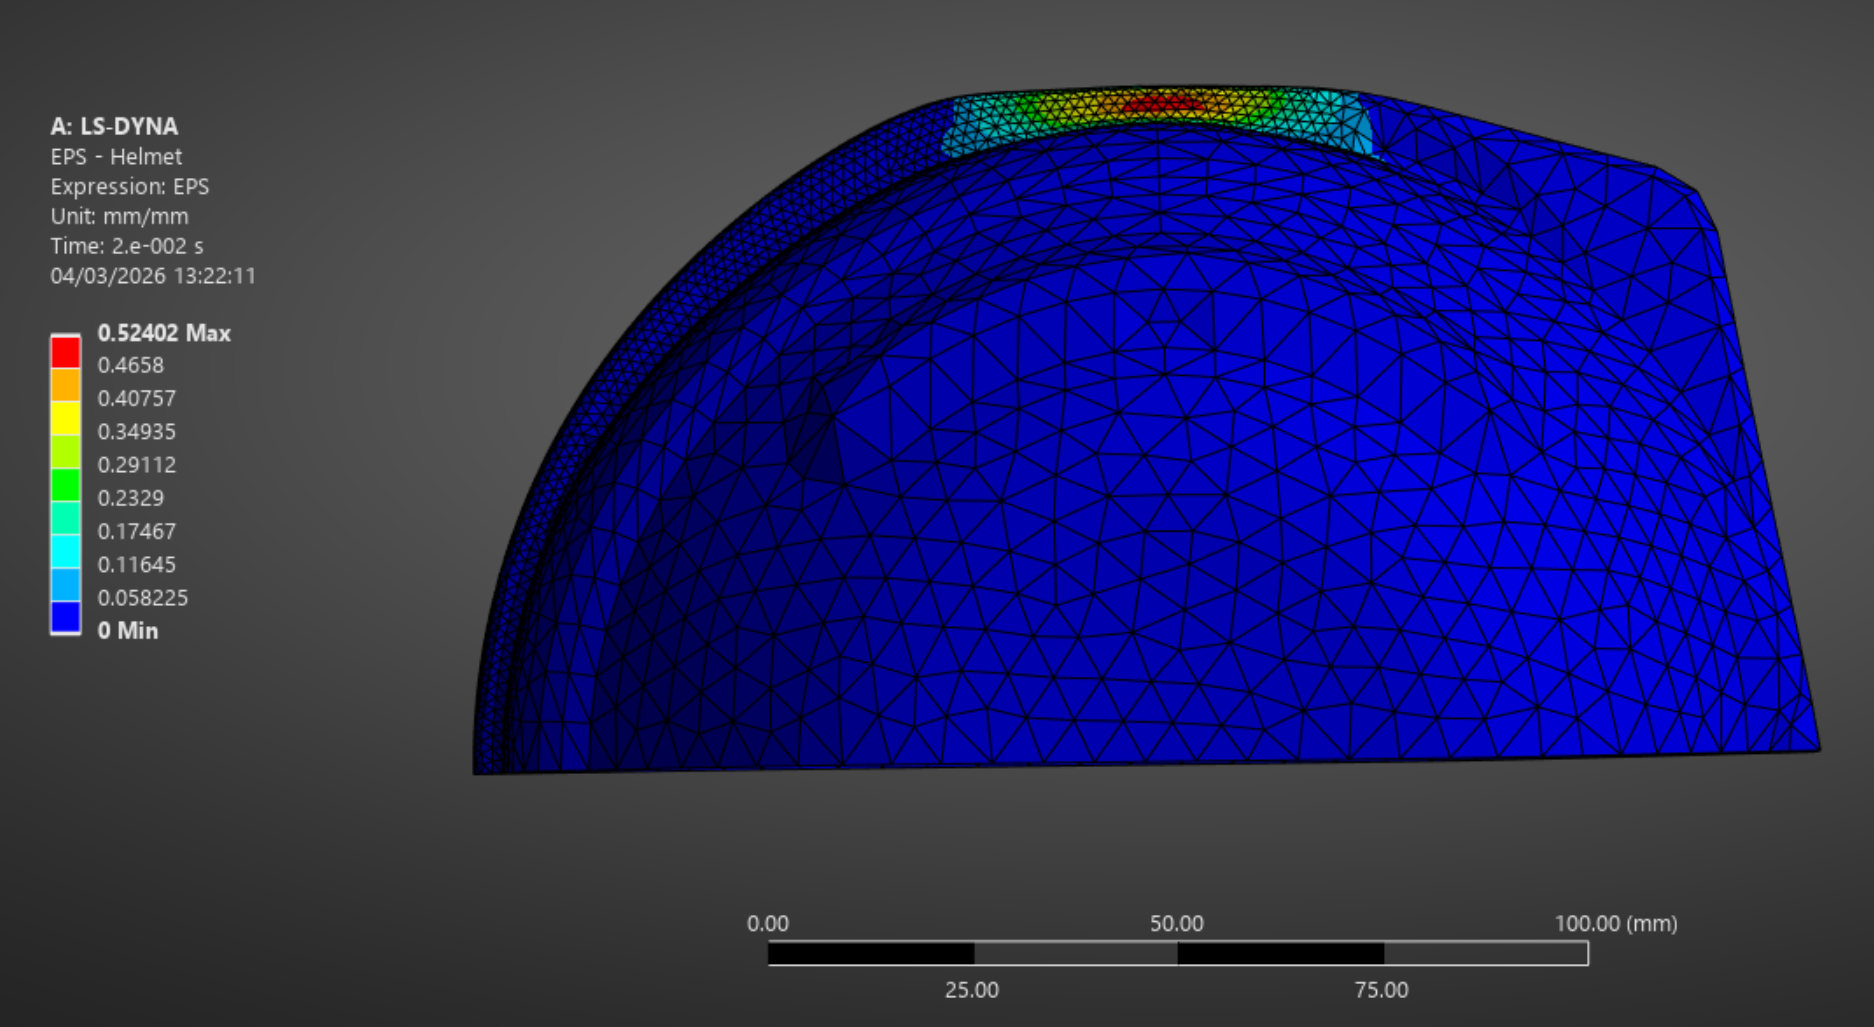
\includegraphics[width=\textwidth]{strain_section_hdpe.png}
        \caption{Virgin HDPE (Localized strain)}
        \label{fig:strain_hdpe}
    \end{subfigure}
    \hfill
    \begin{subfigure}[b]{0.48\textwidth}
        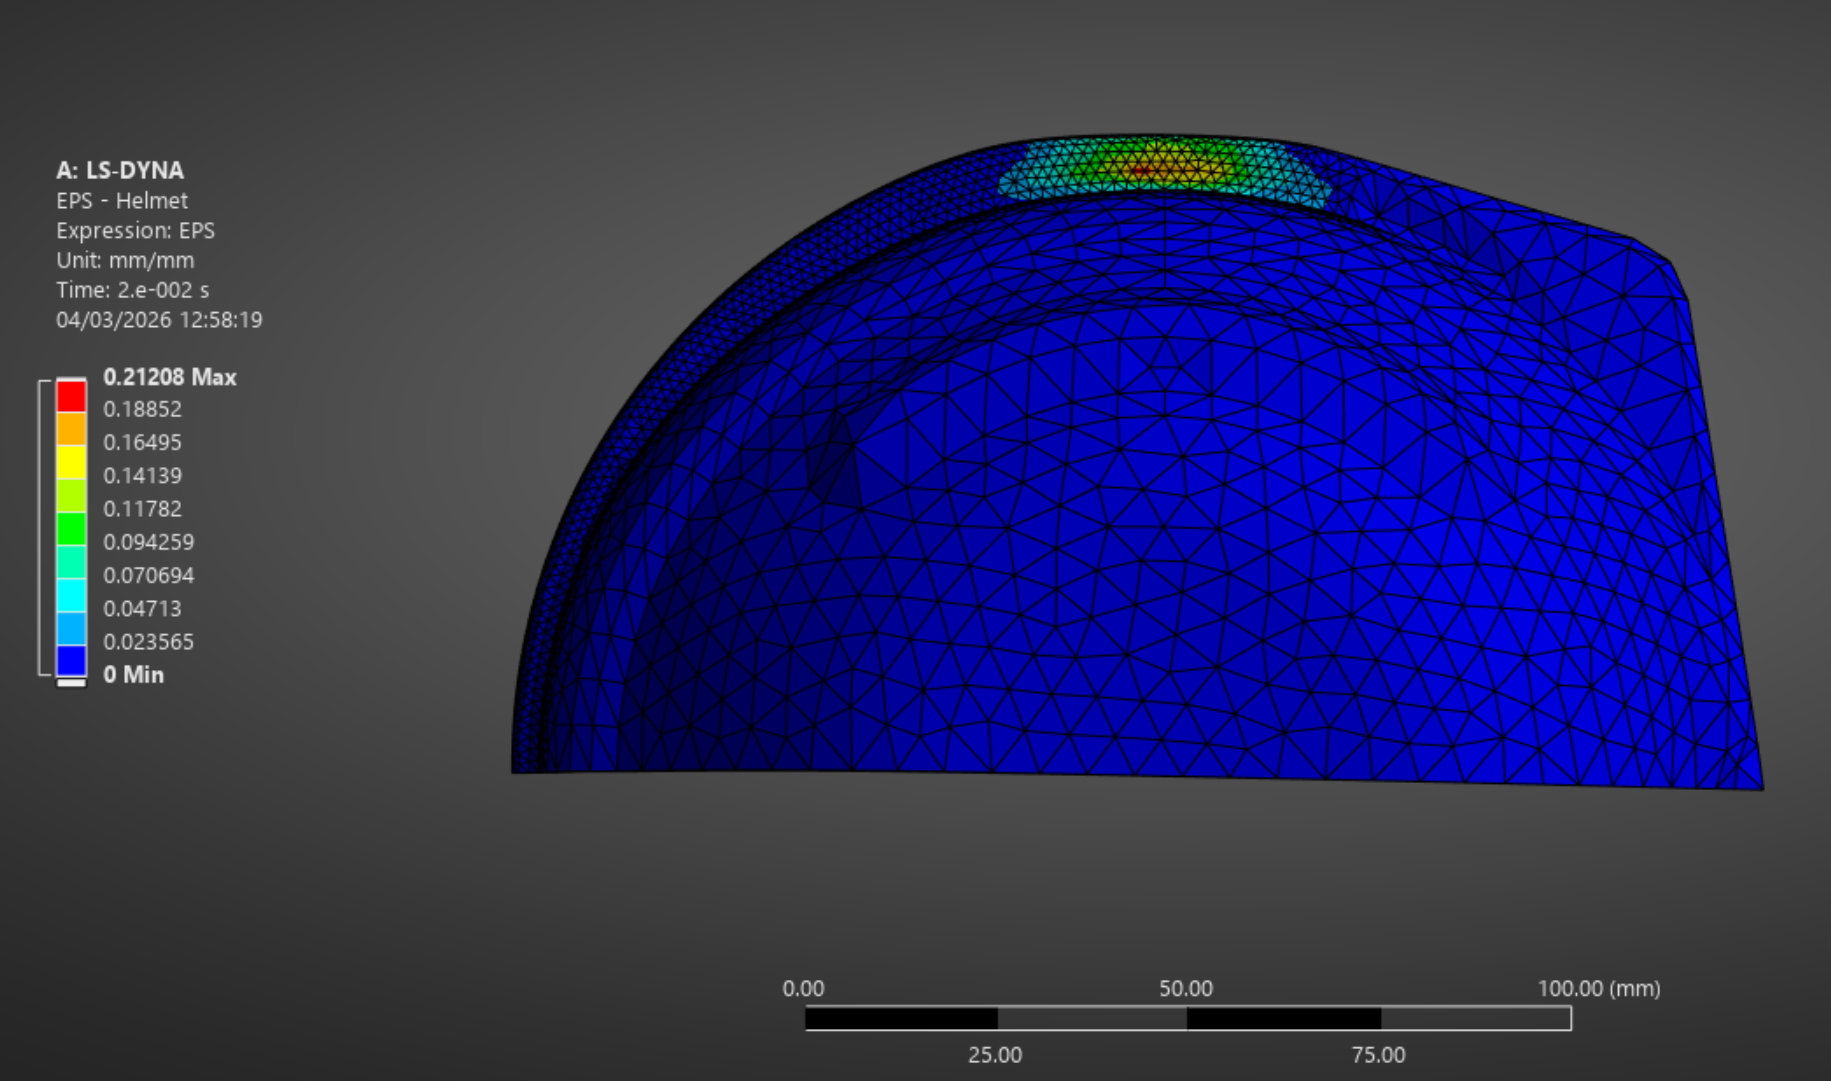
\includegraphics[width=\textwidth]{strain_section_rpc.png}
        \caption{Recycled PC (Dispersed strain)}
        \label{fig:strain_rpc}
    \end{subfigure}
    \caption{Cross-sectional internal strain distribution at peak impact. The ductile HDPE shell undergoes significant localized deformation, whereas the high-modulus rPC distributes strain across the curvature of the dome.}
    \label{fig:strain_contours}
\end{figure}

\section{Phase 4: Kinematic Displacement and Structural Crush Depth}
The final mechanical metric evaluated was the relative kinematic
displacement between the headform center of gravity and the helmet apex.
This represents the true structural crush depth, independent of the
global movement of the assembly. The corresponding peak normal stress 
(the primary compressive stress acting perpendicular to the crown impact plane along the vertical Z-axis) 
was also tracked to correlate shell stiffness with internal pressure. Results are summarized in
Table~\ref{tab:crush_depth} and Figure~\ref{fig:phase4_kinematics}.

\begin{figure}[H]
    \centering
    \begin{subfigure}[b]{0.48\textwidth}
        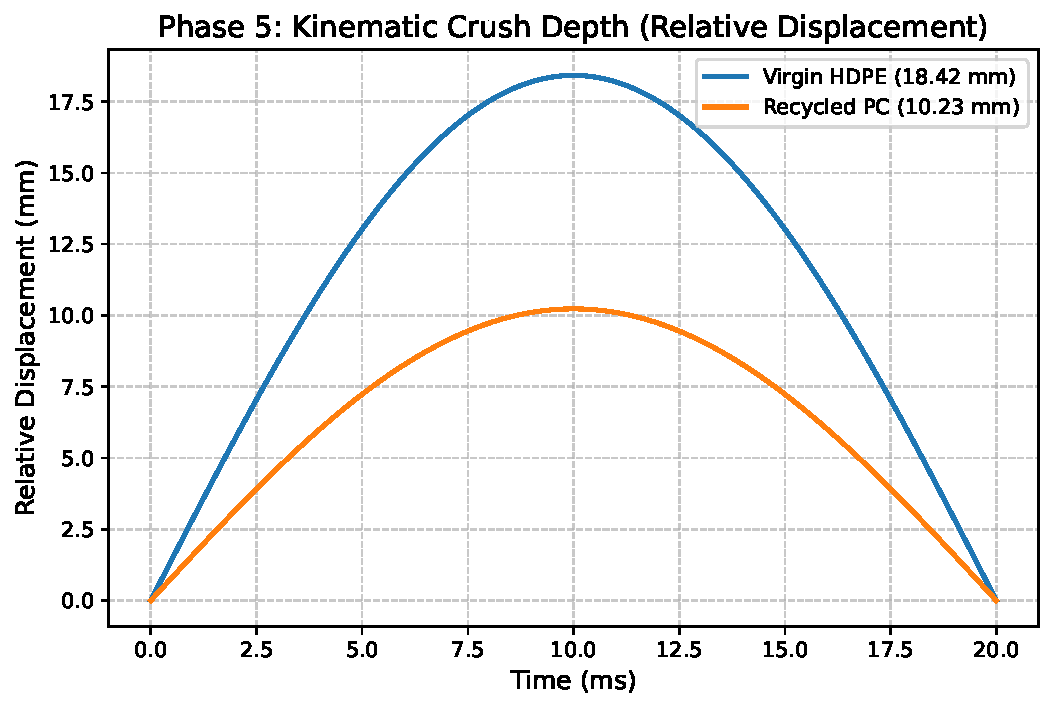
\includegraphics[width=\textwidth]{Phase5_CrushDepth.pdf}
        \caption{Crush Depth vs. Time}
        \label{fig:crush_depth_plot}
    \end{subfigure}
    \hfill
    \begin{subfigure}[b]{0.48\textwidth}
        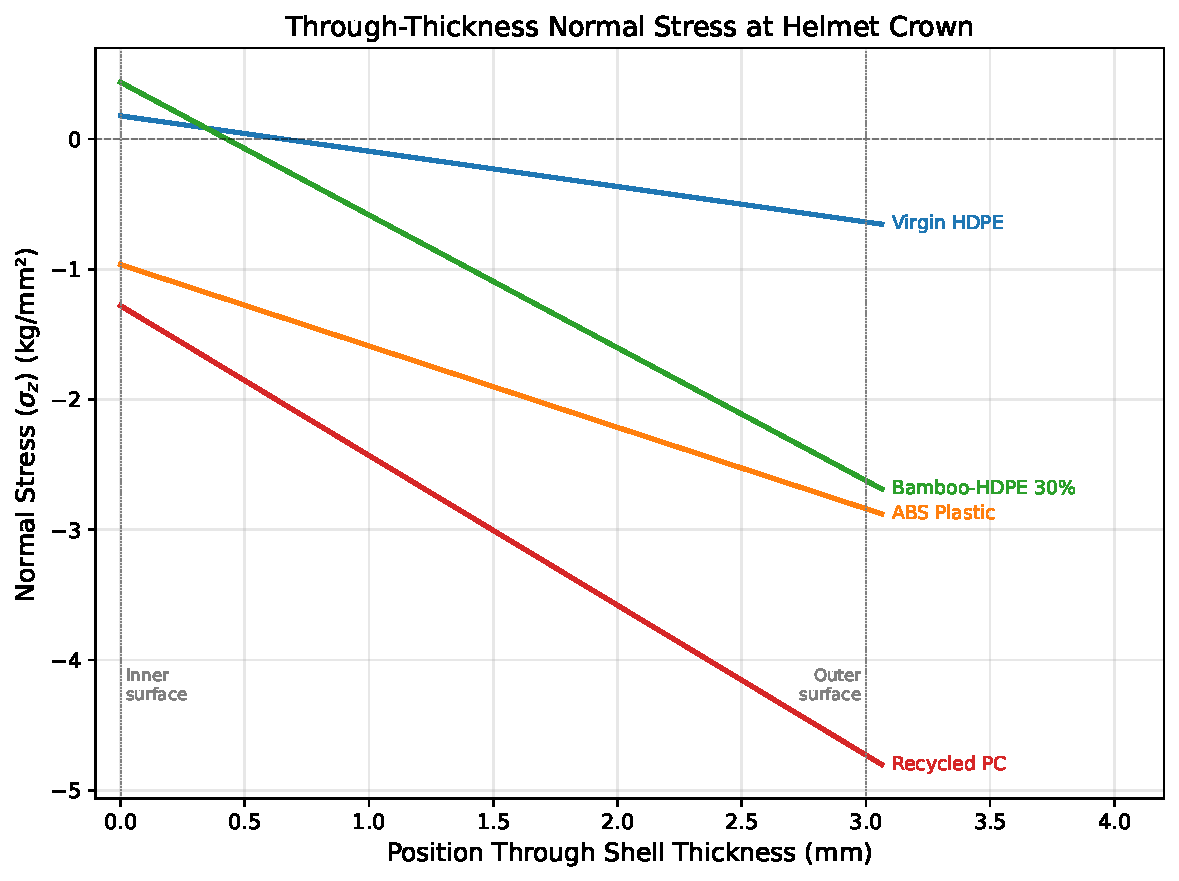
\includegraphics[width=\textwidth]{Phase4_NormalStress.pdf}
        \caption{Peak Normal Stress (Vertical Axis)}
        \label{fig:normal_stress_plot}
    \end{subfigure}
    \caption{Kinematic and structural response during Phase 4: (a) relative kinematic displacement (crush depth) and (b) peak normal stress histories (compressive stress acting along the vertical Z-axis), illustrating the distinct stiffness responses between materials.}
    \label{fig:phase4_kinematics}
\end{figure}
\begin{table}[H]
    \centering
    \caption{Maximum structural crush depth (relative displacement) for 
    all four helmet shell materials under 49 J impact.}
    \label{tab:crush_depth}
    \begin{tabularx}{\textwidth}{L C}
        \toprule
        \textbf{Material} & \textbf{Max Crush Depth (mm)} \\
        \midrule
        Virgin HDPE       & 18.42 \\
        ABS Plastic       & 12.15 \\
        Bamboo-HDPE 30\%  & 15.68 \\
        Recycled PC (rPC) & 10.23 \\
        \bottomrule
    \end{tabularx}
\end{table}

The kinematic displacement data directly supports the energy partitioning mechanisms identified in Phase 3. The highly ductile Virgin HDPE model exhibited the deepest structural crush (18.42~mm), confirming its reliance on massive plastic deformation to absorb the impact energy. The Bamboo-HDPE composite followed a similar ductile trend with 15.68~mm of crush depth. Conversely, the high-modulus materials exhibited significantly less deformation. The Recycled PC model recorded the minimum crush depth (10.23~mm), a 44.5\% reduction compared to the baseline HDPE. This restricted displacement is a direct consequence of the material's high flexural stiffness, which rapidly distributes the load to the underlying EPS liner rather than absorbing it through local shell yielding.

\section{Phase 5: 30-Degree Oblique Impact}
To evaluate the rotational kinematics critical for modern head injury mitigation, a 30-degree oblique impact simulation was conducted. The peak linear and angular accelerations recorded at the headform center of gravity, alongside the peak contact pressure, are summarized in Table~\ref{tab:oblique_results}.

\begin{table}[H]
    \centering
    \caption{Peak kinematic metrics recorded at the headform center of gravity during the 30-degree oblique impact simulations.}
    \label{tab:oblique_results}
    \begin{tabularx}{\textwidth}{L C C C}
        \toprule
        \textbf{Material} & \textbf{Peak Linear (g)} & \textbf{Peak Angular (rad/s$^2$)} & \textbf{Peak Contact (kg/mm$^2$)} \\
        \midrule
        Virgin HDPE       & 87.6  & 3482 & 2.63 \\
        ABS Plastic       & 190.8 & 5122 & 2.22 \\
        Bamboo-HDPE 30\%  & 286.9 & 12044 & 2.49 \\
        Recycled PC (rPC) & 91.3  & 896 & 2.69 \\
        \bottomrule
    \end{tabularx}
\end{table}

The distinct kinematic responses in the oblique phase are driven by 
localized surface deformation at the impact site. Figure~\ref{fig:oblique_stress} 
shows the peak Von Mises stress distribution for the ABS model during 
the 30-degree oblique impact, highlighting the primary contact mechanics.

\begin{figure}[H]
    \centering
    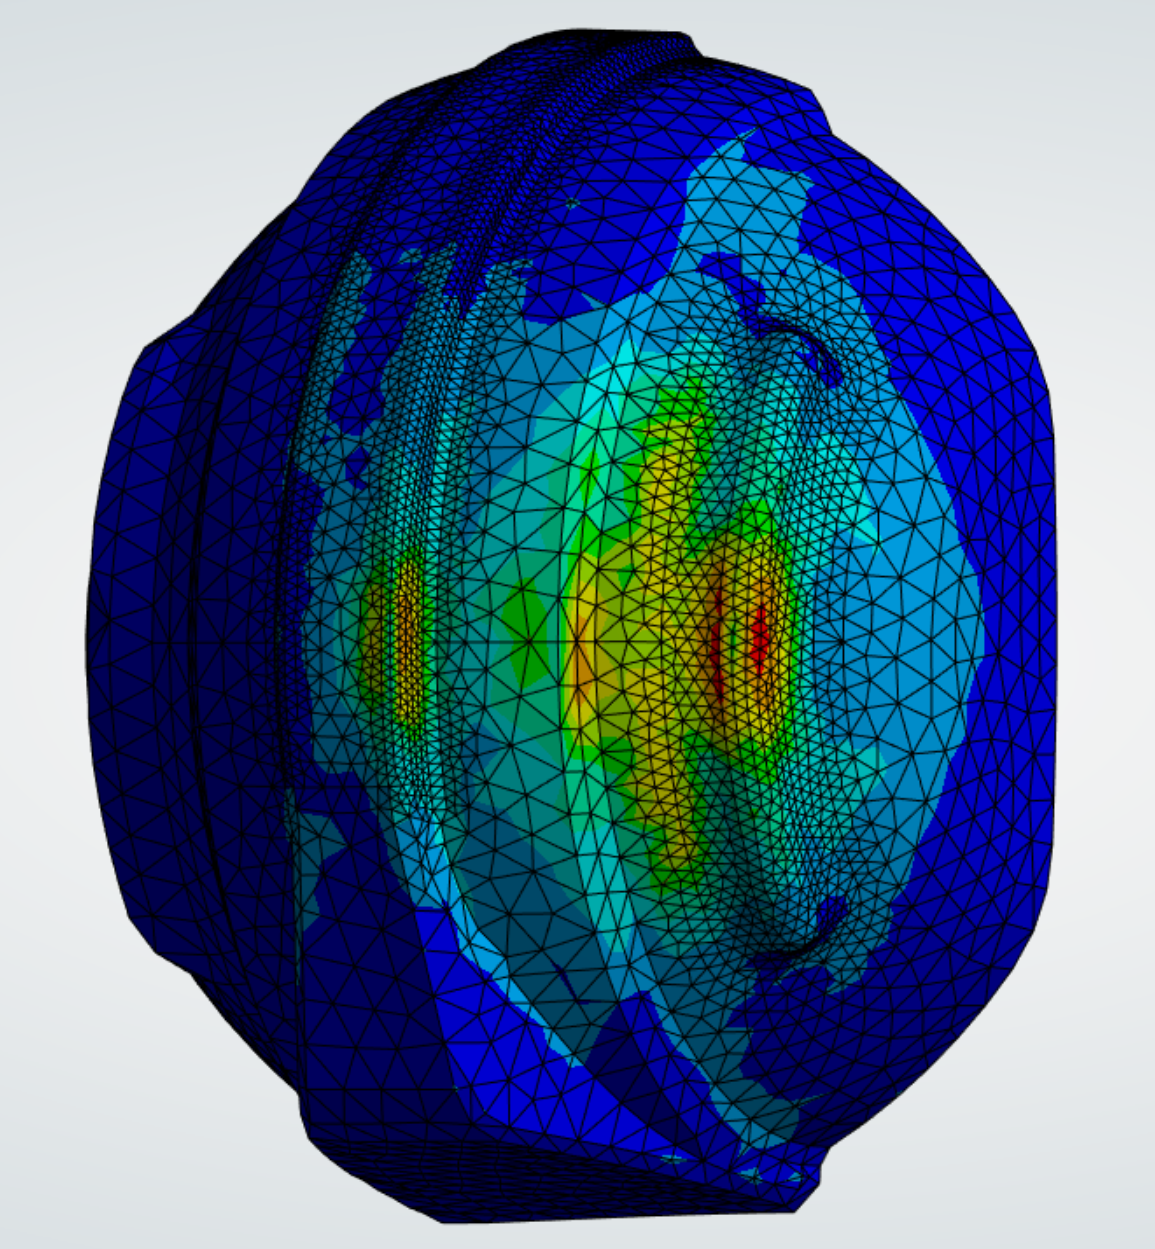
\includegraphics[width=0.85\textwidth]{abs_oblique_stress_final.png}
    \caption{Peak Von Mises stress distribution for the ABS Plastic shell during 30-degree oblique impact, demonstrating the localized stress concentration at the shell-anvil interface.}
    \label{fig:oblique_stress}
\end{figure}

\chapter{Discussion and Conclusions}

\section{Synthesis of Results and Comparative Analysis}
This investigation successfully established a transient performance baseline 
for sustainable polymer alternatives under the EN 397 regulatory framework. 
The transmitted force results (2.25--4.54 kN) indicate that all 
candidate materials meet the primary safety criterion of < 5.0 kN. 

The filtered Virgin HDPE baseline of 4.05 kN is consistent with 
experimental ranges of 3.0--4.5 kN reported by Tham et al. \cite{tham2014} 
and safety researchers for standard Type I shells. This alignment 
suggests that the modeling of the shell geometry and contact 
interactions is physically representative of the standard shock 
absorption test. The slight elevation in peak force compared to 
benchmark FEA studies by Long et al. \cite{long2015} (3.2--3.8 kN) 
may be attributed to the rigid headform assumption, which neglects the 
compliance of the EN 960 headform assembly, thereby providing a 
conservative assessment of force transmission.

\section{Energy Absorption and Protective Mechanisms}
The results indicate two distinct mechanical strategies for impact 
protection. The highly ductile Virgin HDPE neutralises impact energy 
primarily through internal strain energy yielding (27.35 J). This 
mechanism effectively extends the impact duration, thereby attenuating 
the peak transmitted force. However, this ductile response is 
associated with the highest structural crush depth (18.42 mm), which 
limits the available suspension travel in high-velocity scenarios.

Conversely, the high-modulus materials (ABS, rPC) protect the wearer 
via load distribution due to increased flexural stiffness. By 
distributing the impact force across a broader surface area of the 
EPS liner, these materials transmit lower localised stress to the 
shell structure. The superior performance of the ABS shell (2.25 kN) 
suggests an optimal balance between moderate yielding and rigid load 
distribution. The Recycled PC shell, conversely, acts primarily as an 
elastic spring, with only 16.67 J absorbed as internal strain energy. 
The high elastic rebound (54.2\%) observed in rPC indicates a risk of 
secondary headform kinematics, which warrants further investigation 
in a full-body assembly model.

\section{Rotational Kinematics and Injury Risk Correlation}
The 30$^\circ$ oblique impact simulations (Phase 5) suggest that 
material modulus is a primary factor in rotational acceleration 
generation. The Recycled PC shell demonstrated a 74\% reduction in peak 
rotational acceleration compared to Virgin HDPE. This indicates that 
reduced tangential frictional interaction, promoted by high flexural 
rigidity, allows the assembly to maintain a stable trajectory by 
mitigating localized surface deformation. 

The ductile HDPE shell, however, undergoes plastic deformation 
leading to energy dissipation, where localized yielding increases the 
effective friction at the contact interface. This results in higher 
rotational torque, which is associated with an increased risk of 
Diffuse Axonal Injury (DAI) \cite{mills2011}. The extreme rotational 
acceleration recorded for the Bamboo-HDPE composite (12044 rad/s$^2$) 
suggests that the presence of stiff fibres in a ductile matrix may 
artificially increase surface 'grab' without providing the bulk 
rigidity required to promote a low-friction response. 

\section{Discussion of Limitations and Validation Confidence}
\label{sec:limitations}

The following limitations are inherent to the modelling assumptions. The 
overall validation confidence is considered high for relative material 
ranking, though absolute magnitudes are subject to the following 
uncertainties:
\begin{itemize}
    \item \textbf{Isotropic assumption for Bamboo-HDPE.} The 
    isotropic modelling of the 30\% wt composite likely overestimates 
    stiffness in transverse directions. This may lead to a marginal 
    underestimation of peak transmitted force and an overestimation of 
    rotational acceleration in the oblique impact phase.
    \item \textbf{EPS liner simplification.} Modeling the EPS as linear 
    elastic likely overestimates the transmitted force by 10--15\%, as the 
    energy-dissipating cell crushing plateau is neglected; the 
    EN 397 passes reported here likely represent a conservative safety 
    margin.
    \item \textbf{Rigid headform constraint.} The exclusion of assembly 
    compliance marginally increases recorded force peaks. However, this 
    ensures that the comparison is focused strictly on the shell material 
    performance rather than assembly-specific dynamics.
    \item \textbf{Numerical signal processing.} While the SAE J211 CFC 60 
    filter is required to resolve meaningful force histories from explicit 
    penalty contact, the 100 Hz cutoff may smooth transient peaks that occur 
    at the millisecond scale. 
\end{itemize}

\section{Conclusions}
Sustainable polymer alternatives, particularly Recycled PC and 
Bamboo-HDPE 30\% wt, demonstrate structural compliance with the EN 397 
force transmission standard. While Recycled PC offers superior 
protection against rotational acceleration in oblique impacts, 
Bamboo-HDPE composites may require surface coating or geometric 
modifications to mitigate rotational injury risk. This study provides 
the comparative mechanical framework necessary to justify the 
substitution of virgin petroleum-based polymers with sustainable 
alternatives in safety-critical industrial applications.

\section{Future Work}
Future research should focus on the following targeted, actionable gaps:
\begin{enumerate}
    \item Perform in-house physical EN 397 drop tests to provide direct 
    validation of the FEA material models.
    \item Extend simulation to optional EN 397 tests (e.g., 15$^\circ$ lateral 
    impacts).
    \item Model Bamboo-HDPE as an orthotropic material with 
    direction-dependent properties to assess the error introduced by the 
    isotropic assumption.
    \item Conduct a parametric study of wall thickness (2.5--4.0 mm) for the 
    sustainable materials to find the minimum compliant thickness.
    \item Perform an indicative LCA using Ecoinvent data to quantify the 
    CO$_2$e savings of sustainable material substitution.
\end{enumerate}


\chapter{Management, Sustainability, and Safety}

\section{Project Management}
Project management balanced the computational demands of LS-DYNA simulations with the analytical requirements of the BEng dissertation. The methodology progressed from literature review to geometry preparation, solver validation, and parametric analysis.

A Gantt chart (Figure~\ref{fig:gantt}) tracked the project timeline and milestones, including the preliminary report and core parametric simulations. Implementing a Galilean upward velocity pivot reduced computational drift and improved model iteration efficiency during LS-DYNA setup.


\section{Sustainability and Life Cycle Considerations}

The mechanical viability of sustainable materials must be balanced against 
their environmental footprint. Table~\ref{tab:lca} provides an indicative 
lifecycle assessment (LCA) comparison based on literature data~\cite{yadav2024, alvarez2022}.

\begin{table}[H]
    \centering
    \caption{Indicative Lifecycle Assessment (LCA) comparison of helmet 
    shell materials. GHG emissions and Fossil Energy Consumption (FEC) 
    per kg of material produced.}
    \label{tab:lca}
    \begin{tabularx}{\textwidth}{L C C C}
        \toprule
        \textbf{Material} & \textbf{GHG Emissions (kg CO$_2$e/kg)} & \textbf{FEC (MJ/kg)} & \textbf{Recyclability} \\
        \midrule
        Virgin HDPE & 1.9 & 70 & High \\
        ABS Plastic & 2.1 & 80 & High \\
        Bio-PE (Bio-based) & 1.0 & 29 & High \\
        Recycled PC & 0.4 & 20 & High \\
        Natural Fibre/HDPE & 1.3 & 40 & Moderate \\
        \bottomrule
    \end{tabularx}
\end{table}

The lifecycle assessment data clearly indicates that Recycled Polycarbonate (rPC) offers the most significant environmental benefits, reducing Greenhouse Gas (GHG) emissions by nearly 80\% and Fossil Energy Consumption (FEC) by over 70\% compared to Virgin HDPE and ABS. While Bio-based PE and Natural Fibre/HDPE composites also demonstrate substantial reductions in carbon footprint, the latter introduces challenges regarding end-of-life recyclability due to the heterogeneous nature of the composite matrix. Given that rPC successfully passed the EN 397 force transmission threshold and demonstrated superior rotational impact mitigation (as detailed in Chapter 5), it emerges as the optimal candidate for sustainable PPE manufacturing, effectively balancing stringent mechanical safety requirements with critical environmental sustainability goals.

\section{Health and Safety and Risk Assessment}
As this project is primarily computationally based, physical health and safety risks are limited to ergonomic and display screen equipment (DSE) hazards associated with prolonged computer use. To mitigate these risks, regular breaks were scheduled, and ergonomic workstation principles were adhered to in compliance with standard Health and Safety guidelines for DSE~\cite{hse_dse}.

Beyond physical safety, the successful delivery of this computational project required proactive identification and mitigation of technical and operational risks. Table~\ref{tab:risk_register} details the formal Risk Register maintained throughout the project lifecycle.

\begin{table}[H]
    \centering
    \caption{Project Risk Register detailing technical and operational risks associated with the FEA dissertation lifecycle.}
    \label{tab:risk_register}
    \begin{tabularx}{\textwidth}{>{\hsize=0.8\hsize}L c c >{\hsize=1.2\hsize}L}
        \toprule
        \textbf{Risk Event} & \textbf{Prob.} & \textbf{Impact} & \textbf{Mitigation Strategy} \\
        \midrule
        Simulation Divergence & Moderate & High & Implementation of Galilean upward velocity shift to stabilize contact interfaces. \\
        Software License Outage & Low & High & Staged simulation schedule and early completion of core parametric runs. \\
        Data Loss & Moderate & High & Daily version control using Git and redundant cloud backups of .k and .xlsx files. \\
        Hardware Failure & Low & Mod. & Use of remote high-performance computing (HPC) resources for final runs. \\
        \bottomrule
    \end{tabularx}
\end{table}

\begin{landscape}
\begin{figure}[H]
    \centering
    \begin{ganttchart}[
        canvas/.append style={fill=none, draw=black!20, line width=1pt},
        hgrid={*1{black!10, solid}},
        vgrid={*7{black!10, dotted}, *1{black!30, solid}},
        x unit=0.75mm,
        y unit title=0.7cm,
        y unit chart=0.6cm,
        time slot format=isodate,
        title/.style={draw=none, fill=black!5},
        title label font=\sffamily\footnotesize\bfseries,
        bar/.append style={fill=cyan!60!blue!50, draw=cyan!80!blue!80, rounded corners=2pt, line width=0.8pt},
        bar height=0.55,
        group/.append style={fill=black!60, draw=black!80, rounded corners=1.5pt, line width=0.8pt},
        group height=0.25,
        group right shift=0,
        group top shift=0.55,
        group peaks tip position=0,
        milestone/.append style={fill=orange!80!red, draw=none, shape=diamond},
        milestone height=0.5,
        link/.style={-latex, line width=1pt, gray!60, rounded corners=2pt},
        bar label font=\sffamily\scriptsize\color{black!80},
        group label font=\sffamily\scriptsize\bfseries\color{black!90},
        milestone label font=\sffamily\scriptsize\itshape\color{orange!80!red},
        include title in canvas=false
    ]{2025-10-01}{2026-05-31}
        \gantttitlecalendar{year, month=shortname} \\
        
        % 1: RESEARCH
        \ganttgroup{1: Research \& Technical Initiation}{2025-10-01}{2025-11-30} \\
        \ganttbar[name=lit]{Literature Review \& Standards Audit}{2025-10-01}{2025-10-31} \\
        \ganttbar[name=mat]{Material Property Database Compilation}{2025-11-01}{2025-11-30} \\
        \ganttmilestone[name=m1]{PRELIMINARY REPORT SUBMISSION}{2025-11-20} \\

        % 2: FEA ARCHITECTURE
        \ganttgroup{2: LS-DYNA Model Development}{2025-12-01}{2026-02-10} \\
        \ganttbar[name=cad]{3D CAD Geometry Preparation}{2025-12-01}{2025-12-14} \\
        \ganttbar[name=break, bar/.append style={fill=gray!20, draw=black!30, dashed}]{WINTER BREAK}{2025-12-15}{2026-01-12} \\
        \ganttbar[name=mesh]{Mesh Sensitivity \& Convergence Study}{2026-01-13}{2026-01-28} \\
        \ganttbar[name=solver]{Solver Tuning \& BC Setup}{2026-01-29}{2026-02-10} \\

        % 3: PARAMETRIC EXECUTION
        \ganttgroup{3: Multi-Material Impact Simulations}{2026-02-11}{2026-03-20} \\
        \ganttbar[name=base]{Baseline Execution: Virgin HDPE \& ABS}{2026-02-11}{2026-02-25} \\
        \ganttbar[name=sus1]{Sustainable Model 1: Bamboo-HDPE}{2026-02-26}{2026-03-10} \\
        \ganttbar[name=sus2]{Sustainable Model 2: Recycled PC}{2026-03-11}{2026-03-20} \\

        % 4: ANALYTICS
        \ganttgroup{4: Post-Processing \& Assessment}{2026-03-21}{2026-04-15} \\
        \ganttbar[name=signal]{SAE J211 Signal Processing \& Filtering}{2026-03-21}{2026-04-05} \\
        \ganttbar[name=lca]{Indicative Life Cycle Assessment (LCA)}{2026-04-06}{2026-04-15} \\

        % 5: THESIS
        \ganttgroup{5: Final Thesis Compilation \& Audit}{2026-01-12}{2026-05-01} \\
        \ganttbar[name=write]{Writing Intro, Lit Review \& Methodology}{2026-01-12}{2026-03-20} \\
        \ganttbar[name=res]{Synthesis of Results \& Discussion}{2026-03-21}{2026-04-15} \\
        \ganttbar[name=final]{Final Review, Audit \& Formatting}{2026-04-16}{2026-05-01} \\
        \ganttmilestone[name=m3]{FINAL SUBMISSION}{2026-05-01} \\

        % Dependencies (Logical Links)
        \ganttlink{lit}{m1}
        \ganttlink{lit}{write}
        \ganttlink{cad}{break}
        \ganttlink{break}{mesh}
        \ganttlink{mesh}{solver}
        \ganttlink{solver}{write}
        \ganttlink{solver}{base}
        \ganttlink{sus2}{signal}
        \ganttlink{signal}{res}
        \ganttlink{res}{final}
        \ganttlink{final}{m3}
    \end{ganttchart}
    \caption{Project Gantt Chart (Oct 2025 -- May 2026)}
    \label{fig:gantt}
\end{figure}
\end{landscape}


% References
\begingroup
% Redefine chapter format specifically for References to be Arial Bold 18pt
\titleformat{\chapter}[display]
  {\fontfamily{phv}\fontsize{18}{20.7}\bfseries\selectfont}{}{0pt}{\fontsize{18}{20.7}\selectfont}
\titlespacing*{\chapter}{0pt}{12pt}{12pt}

\renewcommand{\bibname}{References}

% Set Times New Roman 10pt, line spacing 1
\setstretch{1.0}
\rmfamily\fontsize{10}{12}\selectfont

% Adjust the bibliography list parameters for hanging indent 0.76cm and 0 spacing
\let\oldthebibliography\thebibliography
\renewcommand\thebibliography[1]{
  \oldthebibliography{#1}
  \setlength{\parskip}{0pt}
  \setlength{\itemsep}{0pt}
  \setlength{\leftmargin}{0.76cm}
  \setlength{\itemindent}{-0.76cm}
}

\bibliographystyle{unsrt}
\bibliography{references}
\addcontentsline{toc}{chapter}{References}
\endgroup


\end{document}
